\documentclass[12pt,a4paper,twoside]{report}
\usepackage[utf8]{inputenc}
\usepackage[spanish,mexico]{babel}
\usepackage{amsmath}
\usepackage{amssymb}
\usepackage{amsthm}
\usepackage{amsfonts}
\usepackage{enumerate}
\usepackage[shortlabels]{enumitem}
\usepackage[dvipsnames]{xcolor}
\usepackage{color,soul}
\definecolor{my_orchid}{rgb}{64,0,64}
\usepackage{pgfplots}
\usepackage[dvipsnames]{xcolor}
\pgfplotsset{compat=1.18, width=10cm}
\usepackage[a4paper, total={6in, 8in}]{geometry}
\usepackage{dsfont}
\usepackage{mathrsfs}
\usepackage{titlepic}
\usepackage{pdfpages}
\usepackage{graphicx}
\usepackage{pgfplots}
\pgfplotsset{width=10cm,compat=1.9}
\usepackage{notes2bib}
\usepackage{blindtext}
\usepackage{hyperref}
\bibliographystyle{unsrt}
\hypersetup{
    colorlinks=true,
    linkcolor=MidnightBlue,
    filecolor=Periwinkle,      
    urlcolor=Skyblue,
    pdftitle={Overleaf Example},
    pdfpagemode=FullScreen,
    }
\urlstyle{same}




\title{\bfseries{Seminario De Geometr\'ia de la Informaci\'on}}
\author{Notas editadas por Aura De la Garza Garc\'ia}
\titlepic{
\includegraphics[width=15cm]{LogoUNAM_IIMAS_Color.png}}
\date{}

\newtheorem{theorem}{Teorema}[section]
\newtheorem{corollary}{Corolario}[theorem]
\newtheorem{lemma}[theorem]{Lema}
\theoremstyle{definition}
\newtheorem{definition}{Definici\'on}[section]
\newtheorem{notation}{Notaci\'on}[section]
\newtheorem{observation}{Observaci\'on}[section]
\newtheorem{example}{Ejemplo}[section]
\renewcommand\qedsymbol{$\blacksquare$}

\usepackage{todonotes}

\newcommand{\alescomment}[1]{\todo[color=red!40]{\small #1 \\ \scriptsize\hfill Ale}}


\begin{document}
\begin{titlepage} 
	\newcommand{\HRule}{\rule{\linewidth}{0.5mm}} 
	
	\center 
	\textsc{\LARGE \textbf{Universidad Nacional Aut\'onoma de M\'exico}}\\[0.9cm] 
	
	\textsc{\Large Instituto de Investigaciones en Matemáticas Aplicadas y Sistemas}\\[0.5cm] 
	
	\textsc{\large Departamento de Matem\'aticas y Mec\'anica}\\[0.5cm] 
	\HRule\\[0.4cm]
	
	{\huge\bfseries Seminario de Geometr\'ia\\
 de la Informaci\'on 2023-2}\\[0.4cm] 
	
	\HRule\\[1cm]
	
	\begin{minipage}{0.4\textwidth}
		\begin{flushleft}
			\large
			\textit{Profesores}\\
			\textsc{Dr. Alessandro Bravetti\\
   Dr. Mario D\'iaz} 
		\end{flushleft}
	\end{minipage}
	~
	\begin{minipage}{0.4\textwidth}
		\begin{flushright}
			\large
			\textit{Asesor de Servicio Social}\\
			\textsc{Dr. Alessandro Bravetti} 
		\end{flushright}
	\end{minipage}
	
    \begin{figure}[htp]
    \centering
    
\includegraphics[width=9.2cm]{LogoUNAM_IIMAS_Color.png}
    \end{figure}
	
	{\large \textit{Notas editadas por} \\ \textsc{Aura De la Garza Garc\'ia}}
 
\end{titlepage}
    \tableofcontents
    \chapter*{Introducci\'on}
    El siguiente trabajo es el resultado de las notas elaboradas para el \textbf{Seminario de Geometr\'ia de la Informaci\'on, Semestre 2023-2}, impartido en el Instituto de Investigaciones en Matem\'aticas Aplicadas y Sistemas. Estas notas fueron creadas como trabajo de servicio social, dentro del programa PAPIIT-IA102823, bajo la asesor\'ia del Dr. Alessandro Bravetti (IIMAS).  
\\

La primera parte de este seminario, impartida por el Dr. Mario D\'iaz (IIMAS), nos presenta una definici\'on formal de \textbf{$f$-divergencias} \cite{1571417125811646464}, en el caso discreto. A lo largo de esta parte, se presentan distintos ejemplos y resultados sobre $f$-divergencias, con el objetivo de presentar m\'etodos matem\'aticos desde una persectiva ”fundamental" para un uso responsable de la privacidad en la informaci\'on con datos a gran escala.

Se comienza por mostrar resultados b\'asicos para $f$-divergencias y se define la privacidad diferencial local. Posteriormente en esta secci\'on, se incluye una demostraci\'on de la Desigualdad de Procesamiento de Informaci\'on \cite{polyanskiy2014lecture}, el cual es uno de los resultados m\'as fundamentales en la Teor\'ia de la Informaci\'on. Por \'ultimo, se definen los Coeficientes de Contracci\'on y con ello, se procede a enunciar la F\'ormula de Dobrushin y dar una demostrac\'ion de la misma. 
\\

La segunda parte del seminario, impartida por el Dr. Alessandro Bravetti, tiene como objetivo dar una breve introducci\'on a la \textbf{Geomet\'ia de la Informaci\'on}. Para lograr un mejor entendimiento de esta rama interdisciplinaria de las matem\'aticas, se comienza por describir esta rama a partir de distintos ejes de estudio. Mientras algunos autores mencionados aqu\'i muestran un enfoque desde las aplicaciones que surgen de esta rama \cite{amari2016information,nielsen2020elementary}, algunos otros autores nos muestran un panorama te\'orico \cite{calin2014geometric,ay2017information} a partir de resultados importantes, como lo es el Teorema Fundamental de la Geometr\'ia de la Informaci\'on~\cite{nielsen2020elementary}, 
o el Teorena de Chentsov~\cite{chentsov1982statiscal}, entre otros que se incluyen en este texto.   

Esta secci\'on, se divide en tres cap\'itulos. En el primer cap\'itulo, se intenta definir y motivar la Geometr\'ia de la Informaci\'on a partir de preguntas que ser\'an respondidas a lo largo del texto. Este cap\'itulo tambi\'en incluye un breve repaso de Inferencia Estad\'istica, donde se mencionar\'an las definiciones y teoremas que m\'as usaremos en esta rama. La segunda parte, consiste en una introducci\'on a algunas herramientas de Geometr\'ia Diferencial que se van a necesitar. En el \'utimo cap\'itulo, utilizando definiciones y resultados que se mostraron en los primeros dos cap\'itulos de esta secci\'on, se muestra una definici\'on formal de una Variedad Estad\'istica, la cual representa el principal objeto de estudio en la Geometr\'ia de la Informaci\'on, y se da una exposici\'on 
del Teorema Fundamental de la Geometr\'ia de la Informaci\'on, el cual nos permite ver a una Variedad Estad\'istica como una generalizaci\'on de una Variedad 
Riemanniana.
\\

Por \'ultimo, cabe resaltar que este trabajo no podr\'a ser utilizado en un proyecto de tesis. El material en este texto se ha elaborado principalmente con el proposito de facilitar futuras consultas en estos temas y reforzar conocimientos en \'areas como Probabilidad, Estad\'istica y Geometr\'ia Diferencial, entre otras. 
    \part{$f$-Divergencias y sus Aplicaciones a la Privacidad}
    \chapter{$f$-Divergencias y Contracci\'on}
    \section{S\'implex de Probabilidad}

\begin{definition}\cite{differentialpriv}
Dada $n\in\mathbb{N}$ el \textbf{\textit{s\'implex de probabilidad}} en $\mathbb{R}^n$ es el conjunto definido por:
\begin{equation}\label{eq:Simplex}
    \mathcal{P}([n]):=\{p\in\mathbb{R}^n\colon p_1,\dots,p_n\geq0,\,p_1+\cdots+p_n=1\}.
\end{equation}
\end{definition}

Para esta definici\'on, tenemos las siguientes observaciones:
\begin{itemize}
    \item $\mathcal{P}([n])$ codifica el conjunto de distribuciones de probabilidad sobre $\{1,2,\dots,n\}$. 
    \item Desde una perspectiva estad\'istica, la geometr\'ia de $\mathcal{P}([n])$ resulta no ser obvia. 
\end{itemize}

\section{$f$-Divergencias I: Definici\'on}

\begin{notation} Como convenci\'on, sea $f\colon(0,\infty)\to\mathbb{R}$ una funci\'on convexa tal que $f(1)=0$
\end{notation}
\begin{notation}
    Cualquier funci\'on de densidad de probailidad a lo largo del texto estar\'a denotada por \textbf{FDP}. Para este seminario, supondremos que las FDP son discretas. Sin embargo, las propiedades que enunciaremos pueden ser generalizadas al caso continuo. 
\end{notation}

\begin{definition}\cite{1571417125811646464}
    Dadas las FDP $P$ y $Q$ la \textbf{\textit{$f$-divergencia}} de $P$ con respecto a $Q$ se define como:
    \begin{equation}\label{eq:fDivergencia}
        D_f(P\|Q)=\sum_{x\in\mathcal{X}}f\left(\frac{P(x)}{Q(x)}\right)Q(x).
    \end{equation}
\end{definition}

\begin{example}\cite{1571417125811646464}
Como ejemplos de $f$-divergencias, tenemos los siguientes:
\begin{enumerate}[label=(\alph*)]
    \item \textbf{Distancia de Variaci\'on total}:
    \begin{equation*}
        f(t)=\frac{1}{2}|t-1|.
    \end{equation*}
    Observemos que, dadas las FDP $P$ y $Q$, tendremos que:
    \begin{align}
    TV(P,Q)&=\sum_{x}f\left(\frac{P(x)}{Q(x)}\right)Q(x)\nonumber\\
    &=\sum_{x}\frac{1}{2}\bigg|\frac{P(x)}{Q(x)}-1\bigg| Q(x)\nonumber\\
    &=\frac{1}{2}\sum_{x}|P(x)-Q(x)|.\label{eq:TV}
    \end{align}
    Adem\'as, notemos la siguiente relaci\'on con la distancia $L^1$: 
    \begin{equation*}
        L^1(P,Q)=\sum_{x}|P(x)-Q(x)|=2\left(\frac{1}{2}\sum_{x}|P(x)-Q(x)|\right)=2\cdot TV(P,Q).
    \end{equation*}
    Dado que $L^1(P,Q)=2\cdot TV(P,Q)$, entonces $TV(P,Q)$ hereda todas las propiedades necesarias para ser una funci\'on distancia. 
    \item \textbf{Divergencia de Hellinger}: 
    \begin{equation*}
        f_\alpha(t)=\frac{t^\alpha-1}{\alpha-1}
    \end{equation*}
    Calculando la divergencia para $\alpha=1/2$, obtendremos que:
    \begin{align}
        H^2(P,Q)&=\sum_x\left(\frac{\sqrt{\frac{P(x)}{Q(x)}}-1}{-1/2}\right)Q(x)\nonumber\\
        &=2-2\sum_x\sqrt{P(x)Q(x)}\,.\label{eq:Hellinger}
    \end{align}
    Se puede notar que en este caso $H^2(P,Q)$ es una distancia. En efecto, pues para $H ^2(P,Q)$ sucede lo siguiente:
    \begin{enumerate}
        \item[(i)] Dado que $P$ y $Q$ son FDP, entonces $P(x)\geq0$ y $Q(x)\geq0$ para toda $x\in\mathcal{X}$. Adem\'as, se tiene que 
        \begin{equation*}
            H^2(P,Q)=2-2\sum_{x}\sqrt{P(x)Q(x)}=2\left(1-\sum_{x}\sqrt{P(x)Q(x)}\right).
        \end{equation*}
        De lo anterior, podemos decir que, 
        \begin{equation*}
            0\leq\sum_{x}\sqrt{P(x)Q(x)}\leq1,
        \end{equation*}
        pues $P$ y $Q$ son FDP. Por lo tanto, se tiene que
        \begin{equation*}
            H^2(P,Q)=2-2\sum_{x}\sqrt{P(x)Q(x)}=2\left(1-\sum_{x}\sqrt{P(x)Q(x)}\right)\geq0.
        \end{equation*}
        Se puede observar que $H^2(P,Q)=0$ si y solo si $P=Q$, pues, si $P=Q$ podemos notar lo siguiente:
        \begin{align*}
            H^2(P,Q)&=2-2\sum_{x}\sqrt{P(x)P(x)}\\
            &=2-2\sum_{x}\sqrt{P^2(x)}\\
            &=2-2\sum_{x}P(x)=2-2=0.
        \end{align*}
        \item[(ii)] Se cumple la propiedad de simetr\'ia, pues para cualuquier $P$ y $Q$ FDP, ocurre lo siguiente:
        \begin{align*}
            H^2(P,Q)&=2-2\sum_{x}\sqrt{P(x)Q(x)}\\
            &=2-2\sum_{x}\sqrt{Q(x)P(x)}\\
            &=H^2(Q,P)
        \end{align*}
        \item[(iii)] Finalmente, para cualquier $P,Q$ y $R$ FDP, se cumple lo siguiente:
        \begin{align*}
            H^2(P,R)&=2-2\sum_{x}\sqrt{P(x)R(x)}\\
            &\leq\left(2-2\sum_{x}\sqrt{P(x)Q(x)}\right)+\left(2-2\sum_{x}\sqrt{Q(x)R(x)}\right)\\
            &=H^2(P,Q)+H^2(Q,R)
        \end{align*}
    \end{enumerate}
    \item \textbf{Divergencia de Kullback-Leibler}: 
    \begin{equation*}
        f(t)=t\log{t}
    \end{equation*}
    Entonces para este caso la divergencia estar\'a dada por:
    \begin{align}
        D_{KL}(P\|Q)&=\sum_x\frac{P(x)}{Q(x)}\log\left(\frac{P(x)}{Q(x)}\right)Q(x)\nonumber\\
        &=\sum_xP(x)\log\left(\frac{P(x)}{Q(x)}\right)\label{eq:KL}
    \end{align}
\end{enumerate}
Como veremos, algunas $f$-divergencias pueden tener operacionalmente interpretaciones \'utiles.  
\end{example}

\section{$f$-Divergencias II: Propiedades B\'asicas}

\begin{theorem}\cite{polyanskiy2014lecture}
Dadas $P$ y $Q$ FDP, se cumplen las siguientes propiedades:
\begin{enumerate}[label=(\alph*)]
    \item $D_f(P\|Q)\geq0$,
    \item Si $f$ es estrictamente convexa en 1, entonces
    \begin{equation*}
        D_f(P\|Q)=0\iff P=Q,
    \end{equation*}
    \item $(P,Q)\mapsto D_f(P\|Q)$ es convexa.
\end{enumerate}
\end{theorem}
\begin{notation}\cite{polyanskiy2014lecture}
    Denotaremos a un \textbf{\textit{Kernel de Markov}} o \textbf{\textit{Mecanismo de Privacidad}} por:
    \begin{equation*}
        K(y|x)=\mathbb{P}(Y=y|X=x).
    \end{equation*}
    Dada una FDP $P$, definimos a $KP$ como:
    \begin{equation*}
        KP(y)=\sum_{x\in\mathcal{X}}P(x)K(y|x)
    \end{equation*}
\end{notation}

\begin{theorem}[\textbf{Desigualdad del Procesamiento de Datos}]\cite{polyanskiy2014lecture}
    Dadas $P$ y $Q$ FDP y una f-divergencia $D_f$, $\forall K$ kernel de Markov se cumple la siguiente desigualdad:
    \begin{equation}\label{eq:DPI}
        D_f(KP\|KQ)\leq D_f(P\|Q).
    \end{equation}
\end{theorem}

\section{$f$-Divergencias III: Divergencia del Palo de Hockey}

\begin{definition}
    Para $\gamma\in(0,\infty)$, la \textbf{\textit{Divergencia del Palo de Hockey}} es la $f$-divergencia definida por:
    \begin{align}\label{eq:Hockey}
         f_\gamma(t)=
         \begin{cases}
             (\gamma-t)_+ &\quad{\gamma<1,}\\
             (t-\gamma)_+ &\quad{\gamma>1},
         \end{cases}
    \end{align}
    donde $(x)_+=\max\{0,x\}$.
    A continuaci\'on denotaremos a esta divergencia por $E_{\gamma}$.
\end{definition}

En la figura~\ref{fig:hockey}, 
podemos ver la gr\'afica de esta funci\'on en el caso de $\gamma=2$. 
Podemos notar que la gráfica tiene forma de un palo de hockey, la cu\'al es la razón de que esta funci\'on reciba este nombre.
\begin{figure}[h!]
\begin{center}
\begin{tikzpicture}[
  declare function={
    func(\x)= (\x <= 2) * (0)   +
              (\x > 2) * (\x-2)
   ;
  }
]
\begin{axis}[
  axis x line=middle, axis y line=middle,
  ymin=0, ymax=6, ytick={0,...,6}, ylabel=$f_\gamma(t)$,
  xmin=0, xmax=6, xtick={0,...,6}, xlabel=$t$,
  domain=0:6,samples=101, 
]

\addplot [Cyan,thick] {func(x)};
\legend{$(t-\gamma)_+$}
\end{axis}
\end{tikzpicture}
\end{center}
\caption{Divergencia del palo de hockey para $\gamma=2$.}\label{fig:hockey}
\end{figure}

\begin{theorem}
    Dadas $P$ y $Q$ FDP, se cumplen las siguientes propiedades:
    \begin{enumerate}[label=(\alph*)]
        \item $\lim_{\gamma\to1}E_\gamma(P\|Q)=TV(P,Q)$,
        \item $\gamma<1$: $E_\gamma(P\|Q)=\sup_{A\subset\mathcal{X}}[\gamma Q(A)-P(A)]$,
        \item $\gamma>1$: $E_\gamma(P\|Q)=\sup_{A\subset\mathcal{X}}[P(A)-\gamma Q(A)]$,
        \item Si $f$ es dos veces diferenciable, entonces
        \begin{equation*}
            D_f(P\|Q)=\int_{0}^{\infty}E_\gamma(P\|Q)f''(\gamma)d\gamma.
        \end{equation*}
    \end{enumerate}
\end{theorem}

\section{$f$-Divergencias IV: Relaci\'on entre $f$-Divergencias}

\begin{theorem}[\textbf{Desigualdad de Pinsker}]
    Dadas $P$ y $Q$ FDP, se cumple la siguiente desigualdad:
    \begin{equation}\label{eq:Pinsker}
        TV(P,Q)\leq\sqrt{\frac{D_{KL}(P\|Q)}{2}}.
    \end{equation}
\end{theorem}

\begin{theorem}
    Dadas $P$ y $Q$ FDP, si $H^2(P,Q)$ es la divergencia de Hellinger
    para $\alpha=2$, ver~\eqref{eq:Hellinger}, entonces
    \begin{equation}\label{eq:H2TVH}
        \frac{1}{2}H^2(P,Q)\leq TV(P,Q)\leq H(P,Q).
    \end{equation}
\end{theorem}

Podemos comenzar a notar que existen muchas relaciones entre $f$-divergencias. 
Sin embargo, en la siguiente secci\'on, veremos que existe una forma sistem\'atica de obtenerlas.  

\section{$f$-Divergencias V: Estrategia del Rango Conjunto}
\begin{definition}\cite{jivri2002lectures}
Un conjunto $C\subseteq\mathbb{R}^d$ es \textbf{\textit{convexo}} si para cualesquiera puntos $x,y\in C$ el segmento $xy$ est\'a totalmene contenido en $C$, es decir, para toda $t\in[0,1]$, se tiene que $tx+(1-t)y\in C$.
\end{definition}

\begin{definition}\cite{jivri2002lectures}
Se define la \textbf{\textit{envolvente convexa}} de un conjunto $X\subseteq\mathbb{R}^d$, denotada por $\text{conv}(X)$, como la itersecci\'on de todos los conjuntos convexos en $\mathbb{R}^d$ que contienen a $X$.   
\end{definition}

\begin{theorem}\cite{jivri2002lectures}
Dado un conjunto $X\subseteq\mathbb{R}^d$, un punto $x$ pertenece a $\text{conv}(X)$ si y solo si existen puntos $x_1,x_2,\dots,x_n\in X$ y reales no negativos $t_1,t_2,\dots,t_n$, con $\sum_{i=1}^{n}t_i=1$, tal que $\sum_{i=1}^{n}t_ix_i=x$.    
\end{theorem}

\begin{notation}\cite{harremoes2011pairs}
    Dadas dos $f$-divergencias $D_f$ y $D_g$, su \textit{\textbf{rango conjunto}} est\'a definido como:
    \begin{align*}
        \mathcal{R}(f,g)&:=\{(D_f(P\|Q),D_g(P\|Q))\colon P,Q\text{ FDP en alg\'un alfabeto $\mathcal{X}$}\},\\
        \mathcal{R}_2(f,g)&:=\{(D_f(P\|Q),D_g(P\|Q))\colon P,Q\text{ FDP en $\{0,1\}$}\}.
    \end{align*}
\end{notation}

\begin{theorem}\cite{harremoes2011pairs}
    Dadas dos funciones convexas $f$ y $g$ se cumple la siguiente igualdad:
    \begin{equation*}
        \mathcal{R}(f,g)=\text{conv}(\mathcal{R}_2(f,g)).
    \end{equation*}
donde $\text{conv}(\mathcal{R}_2(f,g))$, representa la envolvente convexa de $\mathcal{R}_2(f,g)$, seg\'un la Definici\'on 1.6.2.    
\end{theorem}

Como consecuencia de la definici\'on anterior y las desigualdades mencionadas en la secci\'on anterior, se cumple el siguiente teorema:

\begin{theorem}\cite{harremoes2011pairs}
    Dadas $P$ y $Q$ FDP, se cumple la siguiente desigualdad:
    \begin{equation}\label{eq:H2TVHsqrtH}
        \frac{1}{2}H^2(P,Q)\leq TV(P,Q)\leq H(P,Q)\sqrt{1-H^2(P,Q)/4}.
    \end{equation}
\end{theorem}

\section{$f$-Divergencias VI: Desigualdad Fuerte del\\ Procesamiento de Informaci\'on}

\begin{definition}\cite{ahlswede1976spreading,dobrushin1956central}
    El \textit{\textbf{coeficiente de contracci\'on}} de un Kernel de Markov $K$ sobre una $f$-divergencia $D_f$, es definido como:
    \begin{equation}\label{eq:ContractionCoeff}
        \eta_f(K)=\sup_{P,Q:\;0<D_f(P\|Q)<\infty}\frac{D_f(KP\|KQ)}{D_f(P\|Q)}.
    \end{equation}
\end{definition}

\begin{theorem}\cite{ahlswede1976spreading,dobrushin1956central}
    Para toda $P$ y $Q$ FDP se cumple la siguiente desigualdad:
    \begin{equation}\label{eq:StrongDPI}
        D_f(KP\|KQ)\leq\eta_f(K)D_f(P\|Q).
    \end{equation}
\end{theorem}

\begin{theorem}\cite{ahlswede1976spreading,dobrushin1956central}
    Si $K$ es un Kernel de Markov, entonces
    \begin{equation}\label{eq:TVContractionCoeff}
        \eta_{TV}(K)=\sup_{x_1,x_2\in\mathcal{X}}TV(K(\cdot|x_1)\|K(\cdot|x_2)).
    \end{equation}
\end{theorem}

\section{$f$-Divergencias VII: F\'ormula Generalizada de Dobrushin}

\begin{notation}\cite{asoodeh2020contraction,cohen1998comparisons}
    Para mayor facilidad en nuestra notaci\'on, diremos que $\eta_\gamma:=\eta_{E_\gamma}$.
\end{notation}

\begin{theorem}\cite{asoodeh2020contraction,cohen1998comparisons}
Sea $\gamma\in(0,\infty)$. Si $K$ es un Kernel de Markov, entonces:
\begin{equation*}
    \eta_\gamma(K)=\sup_{x_1,x_2\in\mathcal{X}}E_\gamma(K(\cdot|x_1)\|K(\cdot|x_2)).
\end{equation*}
\end{theorem}

\begin{theorem}\cite{asoodeh2020contraction,cohen1998comparisons}
    Si $K$ es un Kernel de Markov, entonces se cumplen las siguientes desigualdades entre coeficientes de contracci\'on:
    \begin{enumerate}[label=(\alph*)]
        \item $\eta_\gamma(K)\leq\eta_{TV}(K)\leq1-\displaystyle{\frac{1-\eta_\gamma(K)}{\gamma}}$ para toda $\gamma\geq1$,
        \item $\eta_f(K)\leq\eta_{TV}(K)$ para toda $f$-divergencia.
    \end{enumerate}
\end{theorem}
    \chapter{Privacidad Diferencial Local}
    \section{Grandes Vol\'umenes de Datos,\\ Grandes Esc\'andalos}

\begin{itemize}
    \item Ignorar la privacidad puede ser problem\'atico.
    \item Distintos escenarios, distintos significados precisos.  
\end{itemize}

\section{Privacidad en Encuestas}

\subsection{Mecanismo de Respuesta Aleatoria}
\begin{enumerate}
    \item Arroje una moneda.
    \item Si se obtiene "\'Aguila" (A), responda honestamente.
    \item Si se obtiene "Sol" (S), entonces arroje la moneda y responda:
    \begin{center}
        \text{"S\'i" si se obtiene Aguila, "No" si se obtiene Sol.}
    \end{center}
\end{enumerate}

\begin{definition}\cite{warner1965randomized}
Para $\varepsilon\geq0$, el \textit{\textbf{mecanismo de respuesta aleatoria}} se define como 
\begin{equation*}
    K(\cdot|0)=\text{Ber}(1-p_\varepsilon)\quad\&\quad K(\cdot|1)=\text{Ber}(p_\varepsilon),
\end{equation*}
donde $p_\varepsilon=e^\varepsilon/(1+e^{\varepsilon})$.
\end{definition}

\section{Privacidad Diferencial Local}

\begin{notation}\cite{evfimievski2003limiting}
Recordemos que $K(A|x)=\mathbb{P}(Y\in A|X=x)$ donde 
\begin{equation*}
    X\rightarrow\fbox{\quad$K$\quad}\rightarrow Y.
\end{equation*}
\end{notation}

\begin{definition}\cite{evfimievski2003limiting}
    Sea $\varepsilon\geq0$ y $\delta\in[0,1]$. Un kernel $K$ es \textit{\textbf{$(\varepsilon,\delta)$-PDL}} (Privacidad Diferencial Local) si para toda $x_1,x_2\in\mathcal{X}$ y $A\subset\mathcal{Y}$,
    \begin{equation*}
        K(A|x_1)\leq e^\varepsilon K(A|x_2)+\delta.
    \end{equation*}
\end{definition}

\begin{itemize}
    \item Para pequeñas $\varepsilon$ y $\delta\in[0,1]$, 
    \begin{equation*}
        |K(y|x_1)-K(y|x_2)|\lesssim\varepsilon+\delta.
    \end{equation*}
    \item La verosimilitud de $y$ dado $x$ no depende mucho de $x$. 
\end{itemize}

\begin{example}\cite{evfimievski2003limiting}
El mecanismo de respuesta aleatoria es $(\varepsilon,0)$-PDL.
\end{example}

\section{Tres Problemas Arquet\'ipicos\\ en An\'alisis de Privacidad}

\begin{itemize}
    \item Entender privacidad desde una persectiva "fundamental". 
    \item Evaluar el costo de privacidad en aplicaciones estad\'isticas espec\'ificas.
    \item Calcular/Estimar los par\'ametros de privacidad de mecanismos espec\'ificos. 
\end{itemize}

\section{PDL como Contracci\'on\\ de la HS-Divergencia}

\begin{observation}\cite{asoodeh2020contraction} Seg\'un lo que definimos en el cap\'itulo anterior, tenemos que:
\begin{itemize}
    \item Representaci\'on de la HS-Divergencia:
    \begin{equation*}
        E_\gamma(P\|Q)=\sup_{A\subset\mathcal{X}}[P(A)-\gamma Q(A)].
    \end{equation*}
    \item F\'ormula Generalizada de Dobrushin:
    \begin{equation*}
        \eta_\gamma(K)=\sup_{x_1,x_2\in\mathcal{X}}E_\gamma(K(\cdot|x_1)\|K(\cdot|x_2)).
    \end{equation*}
\end{itemize}
\end{observation}

\begin{theorem}\cite{asoodeh2020contraction}
Un mecanismo de privacidad $K$ es $(\varepsilon,\delta)$-PDL si y solo si
\begin{equation*}
    \eta_{e^{\varepsilon}}(K)\leq\delta.
\end{equation*}
\end{theorem}
\begin{proof}[\textbf{Demostraci\'on}]
\begin{align*}
    \text{$K$ es $(\varepsilon,\delta)$-PDL}&\iff\sup_{x_1,x_2\in\mathcal{X}}\sup_{A\subset\mathcal{Y}}\left[K(A|x_1)-e^\varepsilon K(A|x_2)\right]\leq\delta\\
    &\iff\sup_{x_1,x_2\in\mathcal{X}}E_{e^\varepsilon}(K(\cdot|x_1)\|K(\cdot|x_2))\leq\delta\\
    &\iff\eta_{e^\varepsilon}(K)\leq\delta.
\end{align*}
\end{proof}

\begin{theorem}[\textbf{Duchi et al. '13}]\cite{asoodeh2020contraction}
Si $K$ es $(\varepsilon,0)$-PDL, entonces
\begin{equation*}
    D_{KL}(KP\|KQ)\leq2(e^\varepsilon-1)^2\|P-Q\|_{TV}.
\end{equation*}
\end{theorem}

\begin{center}
    \textit{"Nuestra t\'ecnica principal...muestra que,\\ aplicando esquemas de muestreo de privacidad diferencial\\
    actua escencialmente como contracci\'on de distribuciones."}
\end{center}

\section{Prueba de Hip\'otesis (Binaria)}
\noindent\textbf{Meta.} De una muestra de $X$ elija entre
\begin{align*}
    &\text{Hip\'otesis Nula}        &H_0: X\sim P.\\
    &\text{Hip\'otesis Alternativa} &H_1:X\sim Q.
\end{align*}

\noindent\textbf{Prueba.} Funci\'on aleatoria $\Psi\colon\mathcal{X}\to\{0,1\}$
\begin{itemize}
    \item Taza Negativa Verdadera
    \begin{equation*}
        \alpha(\Psi):=\mathbb{P}(\Psi(X)=0|H_0).
    \end{equation*}
    \item Taza Negativa Falsa
    \begin{equation*}
        \beta(\Psi):=\mathbb{P}(\Psi(X)=0|H_1).
    \end{equation*}
\end{itemize}

\begin{observation}\cite{polyanskiy2014lecture}
    $\beta_\alpha(P,Q):=\displaystyle{\inf_{\Psi\colon\alpha(\psi)\geq\alpha}\beta(\Psi)}$.
\end{observation}

\section{El costo de PDL en la\\
Prueba de Hip\'otesis Binaria}
\begin{notation}\cite{polyanskiy2014lecture,asoodeh2020contraction}
    Sea $P^{\otimes n}$ la distribuci\'on de 
    \begin{equation*}
        X_1,X_2,\dots,X_n\overset{iid}{\sim}P.
    \end{equation*}
\end{notation}

\begin{lemma}[\textbf{Stein}]\cite{polyanskiy2014lecture,asoodeh2020contraction}
Si $\alpha\in(0,1)$, entonces
\begin{equation*}
    \varliminf _{n\rightarrow \infty }\frac{1}{n}\log\left(\frac{1}{\beta_\alpha(P^{\otimes n},Q^{\otimes n})}\right)=D_{KL}(P\|Q).
\end{equation*}
\end{lemma}
\begin{observation}\cite{polyanskiy2014lecture,asoodeh2020contraction}
Recordemos los siguientes puntos
    \begin{enumerate}[label=(\alph*)]
        \item Bajo $(\varepsilon,\delta)$-PDL: $P\to KP$, $Q\to KQ$ \&
        \begin{equation*}
            D_{KL}(KP\|KQ)\leq\eta_{KL}(K)D_{KL}(P\|Q).
        \end{equation*}
        \item Por la relaci\'on entre $\eta_f$ y $\eta_\gamma$,
        \begin{equation*}
            \eta_{KL}(K)\leq1-\frac{1-\eta_{e^{\varepsilon}}(K)}{e^{\varepsilon}}.
        \end{equation*}
        \item Dado que $K$ es $(\varepsilon,\delta)$-PDL $\iff$ $\eta_{e^{\varepsilon}}(K)\leq\delta$,
        \begin{equation*}
            \eta_{KL}(K)\leq1-\frac{1-\delta}{e^\varepsilon}.
        \end{equation*}
    \end{enumerate}
\end{observation}

\begin{theorem}\cite{polyanskiy2014lecture,asoodeh2020contraction}
    Si $K$ es $(\varepsilon,\delta)$-PDL, entonces
    \begin{equation*}
        \varliminf_{n\to\infty}\frac{1}{n}\log\left(\frac{1}{\beta_\alpha(KP^{\otimes n},KQ^{\otimes n})}\right)\leq\left(1-\frac{1-\delta}{e^\varepsilon}\right)D_{KL}(P\|Q).
    \end{equation*}
\end{theorem}
\section{Privacidad Diferencial (PD)\\
bajo Composici\'on:\\
Algoritmos Iterativos}

\begin{equation*}
    \mu_0\sim W_0\to\fbox{\fbox{$K_1$}$\to$\fbox{$K_2$}$\to\cdots\to$\fbox{$K_n$}}\to W_n\sim\mu_n
\end{equation*}

\begin{itemize}
    \item PD para algoritmos iterativos:
    \begin{equation*}
        \sum_{\mu_0,\mu_0'\in\mathcal{P}(\mathcal{X})}E_{\gamma}(\mu_n\|\mu_n')\leq\delta\quad\text{con}\quad\gamma=e^\varepsilon.
    \end{equation*}
    \item Filosof\'ia de Contracci\'on:
    \begin{equation*}
        E_\gamma(\mu_n\|\mu_n')\leq\eta_{E_\gamma}(K_n)\cdot\eta_{E_\gamma}(K_1).
    \end{equation*}
\end{itemize}

\begin{example}[\textbf{Descenso del Gradiente Estoc\'astico}]
\begin{equation*}
    W_{t+1}=W_t-\eta\nabla f_t(W_t)+\sigma Z_{t+1}
\end{equation*}
\begin{itemize}
    \item $\eta,\sigma>0$,
    \item $t_1,\dots,t_n$ "Funciones de P\'erdida",
    \item $Z_1,\dots,Z_n$ \textit{i.i.d.} normales.
\end{itemize}
\end{example}

\section{\'Ultimas Observaciones}

Seg\'un la teor\'ia que hemos desarrollado, podemos decir que los problemas arquet\'ipicos en el an\'alisis de privacidad, ahora son los siguientes:

\begin{itemize}
    \item Entender privacidad desde una persectiva "fundamental". 
    \item Evaluar el costo de privacidad en aplicaciones estad\'isticas espec\'ificas.
    \item Calcular/Estimar los par\'ametros de privacidad de mecanismos espec\'ificos. 
    \item Proporcionar evidencia estadistica de implementaci\'on incorrecta. 
\end{itemize}

    \chapter{Demostraci\'on de la Desigualdad\\ del Procesamiento de Informaci\'on}
    \section{Recapitulaci\'on de
Cap\'itulos Previos}

\begin{notation}
$\mathcal{P}(\mathcal{X})$ denota las distribuciones de probabilidad en un conjunto $\mathcal{X}$. Por ahora, solamente trabajaremos con distribuciones discretas, pero existe una forma de generalizar estos conceptos para distribuciones continuas.
\end{notation}

\begin{example}
$\mathcal{X}=\{0,1\}$
\begin{equation*}
    \mathcal{P}(\mathcal{X})=\{\text{Ber}(p)\colon p\in[0,1]\},
\end{equation*}
donde $X\sim\text{Ber}(p)$,
\begin{equation*}
    \mathbb{P}(X=1)=p,\quad\mathbb{P}(X=0)=1-p=\bar{p}.
\end{equation*}
\end{example}

\begin{definition}
Sea $f\colon(0,\infty)\to\mathbb{R}$ una funci\'on convexa con $f(1)=0$. La \textit{\textbf{$f$-divergencia}} de $P$ respecto a $Q$ ($P,Q\in\mathcal{P}(\mathcal{X})$), se define como
\begin{equation*}
    D_f(P\|Q)=\sum_{x\in\mathcal{X}}f\left(\frac{P(x)}{Q(x)}\right)Q(x).
\end{equation*}
\end{definition}

\begin{observation}
Una idea intuitiva de la definici\'on anterior es medir qu\'e tan distintas son las distribuciones. 
\end{observation}

\begin{example}[\textbf{KL-Divergencia}]
\begin{equation*}
    f(t)=t\log(t).
\end{equation*}
\end{example}

\begin{observation}
    Si $X\sim Q$, entonces:
    \begin{equation*}
        D_f(P\|Q)=\mathbb{E}\left[f\left(\frac{P(x)}{Q(x)}\right)\right]
    \end{equation*}
    lo cual, es una forma alternativa de interpretar una $f$-Divergencia.
\end{observation}

\begin{example}
Para la KL-Divergencia, tendremos que:
\begin{align*}
    D_{KL}(P\|Q)&=\sum_{x\in\mathcal{X}}\frac{P(x)}{Q(x)}\log\left(\frac{P(x)}{Q(x)}\right)Q(x)\\
    &=\sum_{x\in\mathcal{X}}P(x)\log\left(\frac{P(x)}{Q(x)}\right).
\end{align*}
\end{example}
\section{Propiedades de $f$-Divergencias}
\begin{example}
    Si $X_1$ y $X_2$ son independientes
    \begin{align*}
        P&=P_{X_1}(x_1)P_{X_2}(x_2)\\
        Q&=Q_{X_1}(x_1)Q_{X_2}(x_2)
    \end{align*}
    entonces:
    \begin{align*}
        D_{KL}(P_{X_1}P_{X_2}\|Q_{X_1}Q_{X_2})&=\sum_{x_1}\sum_{x_2}P_{X_1}(x_1)P_{X_2}(x_2)\log\left(\frac{P_{x_1}(x_1)P_{X_2}(x_2)}{Q_{X_1}(x_1)Q_{X_2}(x_2)}\right)\\
        &=\sum_{x_1}\sum_{x_2}P_{X_1}(x_1)P_{X_2}(x_2)\log\left(\frac{P_{X_1}(x_1)}{Q_{X_1}(x_1)}\right)\\
        &\quad+\sum_{x_1}\sum_{x_2}P_{X_1}(x_1)P_{X_2}(x_2)\log\left(\frac{P_{X_2}(x_2)}{Q_{X_2}(x_2)}\right)\\
        &=\sum_{x_1}P_{X_1}(x_1)\log\left(\frac{P_{X_1}(x_1)}{Q_{X_1}(x_1)}\right)\\
        &\quad+\sum_{x_2}P_{X_2}(x_2)\log\left(\frac{P_{X_2}(x_2)}{Q_{X_2}(x_2)}\right)\\
        &=D_{KL}(P_{X_1}\|Q_{X_1})+D_{KL}(P_{X_2}\|Q_{X_2}).
    \end{align*}
\end{example}

\begin{theorem}[\textbf{Tensorizaci\'on}]
Si $X_1,\dots,X_n$ son variables aleatorias independientes, entonces:
\begin{equation*}
    D_{KL}(P_{X_1}\cdots,P_{X_n}\|Q_{X_1},\cdots,Q_{X_n})=\sum_{i=1}^{n}D_{KL}(P_{X_i}\|Q_{X_i}).
\end{equation*}
\end{theorem}

\begin{example}[\textbf{Variaci\'on Total}]
 \begin{equation*}
     f(t)=\frac{1}{2}|t-1|.
 \end{equation*}
Su $f$-divergencia estar\'a dada por:
\begin{align*}
    TV(P,Q)&=\sum_{x\in\mathcal{X}}\frac{1}{2}\bigg|\frac{P(X)}{Q(x)}-1\bigg|Q(x)\\
    &=\frac{1}{2}\sum_{i=1}^{n}|P(x)-Q(x)|.
\end{align*}
\end{example}

\begin{observation}[\textbf{Kernel de Markov}]
\begin{equation*}
    X\to\fbox{$K$}\to Y
\end{equation*}
\begin{equation*}
    \underbrace{{K(y|x)}=\mathbb{P}(Y=y|X=x)=\mathbb{P}_{Y|X}(y|x)}_{\textrm{Matriz de Transici\'on (Cadenas de Markov)}}
\end{equation*}
\end{observation}

\begin{notation}
        \begin{align*}
            P_{X}P_{Y|X}(x,y)&=P_{X}(x)P_{Y|X}(y|x)\\
            &=\mathbb{P}(X=x,Y=y)
        \end{align*}
\end{notation}
\begin{notation}
        \begin{align*}
            (P_{Y|X}P_{X})(y)=\sum_{x\in\mathcal{X}}P_{Y|X}(y|x)P_{X}(x)=\mathbb{P}(Y=y).
        \end{align*}
\end{notation}
\section{$f$-Divergencia Condicional
y Propiedades B\'asicas}
\begin{definition}
    Sean $P_{Y|X}$ y $Q_{Y|X}$ dos Kerneles. Su \textit{\textbf{$f$-divergencia condicional}} dada $P_{X}\in\mathcal{P}(\mathcal{X})$, se define:
    \begin{equation*}
        D_f(P_{Y|X}\|Q_{Y|X}|P_{X})
    \end{equation*}
\end{definition}
\begin{observation}
Observemos que de la definici\'on anterior, se sigue que:
\begin{align*}
    D_f(P_{Y|X}\|Q_{Y|X}|P_{X})&=\sum_{x\in\mathcal{X}}P_{X}(x)D_f\bigl(P_{Y|X}(\cdot|x)\big\|Q_{Y|X}(\cdot|x)\bigl)\\
    &=\sum_{x\in\mathcal{X}}P_{X}(x)\sum_{y\in\mathcal{Y}}f\left(\frac{P_{Y|X}(y|x)}{Q_{Y|X}(y|x)}\right)Q_{Y|X}(y|x)\\
    &=\sum_{x}\sum_{y}f\left(\frac{P_{Y|X}(y|x)}{Q_{Y|X}(y|x)}\right)P_X(x)Q_{Y|X}(y|x)\\
    &=\sum_{x}\sum_{y}f\left(\frac{P_{Y|X}(y|x)}{Q_{Y|X}(y|x)}\cdot\frac{P_X(x)}{P_X(x)}\right)P_X(x)Q_{Y|X}(y|x)\\
    &=D_f(P_XP_{Y|X}\|P_XQ_{Y|X}).
\end{align*}
Por lo tanto, la definici\'on anterior, nos dice que:
\begin{equation*}
    D_f(P_{Y|X}\|Q_{Y|X}|P_{X})=D_f(P_XP_{Y|X}\|P_XQ_{Y|X}).
\end{equation*}
\end{observation}
\begin{theorem}[\textbf{Desigualdad de Jensen}]
    Dada $Z$ una variable aleatoria y $f$ una funci\'on convexa, se cumple la siguiente desigualdad:
    \begin{equation*}
        \mathbb{E}\left[f(Z)\right]\geq f(\mathbb{E}(Z)).
    \end{equation*}
\end{theorem}

\begin{theorem}
    Sea $f\colon(0,\infty)\to\mathbb{R}$ una funci\'on convexa con $f(1)=0$, $P$ y $Q$ FDP. Entonces, se cumplen las siguientes propiedades:
    \begin{enumerate}[label=(\alph*)]
        \item $D_f(P\|Q)\geq0$,
        \item Si $f$ es estrictamente convexa en 1, entones:
        \begin{equation*}
            D_f(P\|Q)=0\iff P=Q,
        \end{equation*}
        \item $(P,Q)\mapsto D_f(P\|Q)$ es convexa,
        \item $D_f(P_{Y|X}P_X\|Q_{Y|X}P_X)\leq D_f(P_XP_{Y|X}\|P_XQ_{Y|X})$.
    \end{enumerate}
\end{theorem}
\begin{proof}[\textbf{Demostraci\'on}]
\begin{enumerate}[label=(\alph*)]
    \item Observemos que:
    \begin{align*}
        D_f(P\|Q)&=\sum_xf\left(\frac{P(x)}{Q(x)}\right)Q(x)\\
        &\geq f\left(\sum_{x}\frac{P(x)}{Q(x)}\cdot Q(x)\right)\quad\text{Desigualdad de Jensen}\\
        &=f(1)=0.
    \end{align*}
    \textit{Demostraci\'on Alternativa}: Sea $Z=\frac{P(x)}{Q(x)}$ con $X\sim Q$. Observemos que:
    \begin{align*}
        D_f(P\|Q)&=\mathbb{E}\left[f\left(\frac{P(x)}{Q(x)}\right)\right]\quad(X\sim Q)\\
        &=\mathbb{E}[f(Z)]\\
        &\geq f(\mathbb{E}(Z))\quad\text{(Desigualdad de Jensen)}
    \end{align*}
    Puesto que $\mathbb{E}[Z]=\sum_{x\in\mathcal{X}}\frac{P(x)}{Q(x)}$, donde $Q(x)=1$, entonces, concluimos que:
    \begin{equation*}
        D_f(P\|Q)\geq f(1)=0.
    \end{equation*}
    \item Basta con aplicar la condici\'on de igualdad para la Desigualdad de Jensen.
    \item Definamos $g:(0,\infty)^2\to\mathbb{R}$ por
    \begin{equation*}
        g(p,q)=q\cdot f\left(\frac{p}{q}\right).
    \end{equation*}
    Observemos que:
    \begin{equation*}
        D_f(P\|Q)=\sum_{x\in\mathcal{X}}f\left(\frac{P(x)}{Q(x)}\right)Q(x)=\sum_{x\in\mathcal{X}}g(P(x),Q(x)).
    \end{equation*}
    Se puede demostrar que $g$ es convexa, \textit{i.e.} $\forall (p_1,q_1),(p_2,q_2)$ y $\lambda\in(0,1)$, se cumple que:
    \begin{equation*}
        g(\lambda p_1+\bar{\lambda}p_2,\lambda q_1+\bar{\lambda}q_2)\leq \lambda g(p_1,q_1)+\bar{\lambda}g(p_2,q_2).
    \end{equation*}
    Por lo tanto, para $\lambda\in[0,1]$
    \begin{align*}
        \lambda D_f(P_1\|Q_1)+\bar{\lambda}D_f(P_2\|Q_2)
        &=\sum_{x}\Bigl\{\lambda g(P_1(x),Q_1(x))+\sum_{x}\bar{\lambda}g(P_2(x),Q_2(x))\Bigl\}\\
        &=\sum_{x}g\left(\lambda P_1(x)+\bar{\lambda}P_2(x),\lambda Q_1(x)+\bar{\lambda}Q_2(x)\right)\\
        &=D_f(\lambda P_1+\bar{\lambda}P_2\|\lambda Q_1+\bar{\lambda}Q_2)
    \end{align*}
    \item Observemos que 
    \begin{align*}
        D_f(P_XP_{Y|X}\|P_XQ_{Y|X})&=D_f(P_{Y|X}\|Q_{Y|X}|P_X)\\
        &=\sum_{x\in\mathcal{X}}P_X(x)D_f\left(P_{Y|X}(\cdot|x)\|Q_{Y|X}(\cdot|x)\right)\\
        &\quad\text{(por (c): Convexidad )}\\
        &\geq D_f\left(\sum_xP_{Y|X}(\cdot|x)P_X(x)\Bigg\|\sum_xQ_{Y|X}(\cdot|x)P_X(x)\right)\\
        &=D_f(P_{Y|X}P_X\|Q_{Y|X}P_X)
    \end{align*}
\end{enumerate}
\end{proof}

\section{Demostraci\'on de la Desigualdad del\\
Procesamiento de Informaci\'on (DPI)}

\noindent Finalmente, con todas las herramientas que hemos desarrollado, daremos una demostraci\'on de la Desigualdad del Procesamiento de la Informaci\'on

\begin{theorem}[\textbf{Desigualdad del Procesamiento de Informaci\'on}]
Si $P_{Y|X}$ es un Kernel, entonces
\begin{equation*}
    D_f(P_{Y|X}P_X\|P_{Y|X}Q_{X})\leq D_f(P_X\|Q_X).
\end{equation*}
Suponiendo que $K=P_{Y|X}$ tal que:
\begin{align*}
    P_X&\to\fbox{$K$}\to P_Y\\
    Q_X&\to\fbox{$K$}\to Q_Y
\end{align*}
la desigualdad se reduce a lo siguiente:
\begin{equation*}
    D_f(P_Y\|Q_Y)\leq D_f(P_X\|Q_X)
\end{equation*}
\end{theorem}
\begin{proof}[\textbf{Demostraci\'on}]
Observemos que
\begin{align*}
    D_f(P_X\|Q_X)&=\sum_{x}f\left(\frac{P_X(x)}{Q_X(x)}\right)Q_X(x)\\
    &=\sum_x\sum_y f\left(\frac{P_X(x)}{Q_X(x)}\right)Q_X(x)P_{Y|X}(y|x)\\
    &=\sum_x\sum_y f\left(\frac{P_X(x)P_{Y|X}(y|x)}{Q_X(x)P_{Y|X}(y|x)}\right)Q_X(x)P_{Y|X}(y|x).
\end{align*}
Observemos que
\begin{align*}
    Q_Y(x)P_{Y|X}(y|x)&=Q_{X,Y}(x,y)\\
    &=Q_Y(y)Q_{X|Y}(x|y)
\end{align*}
puesto que
\begin{equation*}
    Q_{X|Y}(x,y)=\frac{Q_{X,Y}(x,y)}{Q_Y(y)}
\end{equation*}
Por lo tanto,
\begin{align*}
    D_f(P\|Q)&=\sum_x\sum_y f\left(\frac{P_{X,Y}(x,y)}{Q_{X,Y}(x,y)}\right)Q_Y(y)Q_{X|Y}(x|y)\\
    &=\sum_y Q_Y(y)\sum_x f\left(\frac{P_{X,Y}(x,y)}{Q_{X,Y}(x,y)}\right)Q_{X|Y}(x|y)\\
    &\geq\sum_y Q_Y(y) f\left(\sum_{x}\frac{P_{X,Y}(x,y)}{Q_{X,Y}(x,y)}\cdot\frac{Q_{X,Y}(x,y)}{Q_Y(y)}\right)\\
    &=\sum_y Q_Y(y) f\left(\frac{P_Y(y)}{Q_Y(y)}\right)\\
    &=D_f(P_Y\|Q_Y).
\end{align*}
\end{proof}

Observemos que, este teorema nos dice que, estad\'isticamente, el post-procesamiento de informaci\'on no puede incrementar nuestra informaci\'on inicial. Este es un teorema que tiene muchas implicaciones dentro de la Teor\'ia de la Informaci\'on.
    \chapter{F\'ormulas Variacionales\\
    para las Divergencias $TV$ y $KL$}
    \section{Recapitulaci\'on de\\
Cap\'itulos Previos}

\begin{itemize}
    \item $f\colon(0,\infty)\to\mathbb{R}$ con $f(1)=0$ y $f$ convexa.
    \item Para $P,Q\in\mathcal{P}(\mathcal{X})$, se define su \textbf{$f$-divergencia} como
    \begin{equation*}
        D_f(P\|Q)=\sum_{x\in\mathcal{X}}f\left(\frac{P(x)}{Q(x)}\right)Q(x).
    \end{equation*}
    \item \textbf{Kernel de Markov}: $K(y|x)=\mathbb{P}(Y=y|X=x)$
    \begin{equation*}
        X\to\fbox{$K$}\to Y.
    \end{equation*}
    \item \textbf{$f$-Divergencia Condicional} de $P_{Y|X}$ y $Q_{Y|X}$ dada $P_X$ se define como
    \begin{align*}
        D_f(P_{Y|X}\|Q_{Y|X}|P_X)=\sum_{x\in\mathcal{X}}P_X(x)D_f(P_{Y|X}(\cdot|x)\|Q_{Y|X}(\cdot|x))
    \end{align*}
    \item Propiedades de las $f$-divergemcias:
    \begin{enumerate}[label=(\alph*)]
        \item $D_f(P\|Q)\geq0$,
        \item $(P,Q)\mapsto D_f(P\|Q)$ es convexa,
        \item \textbf{Desigualdad del Procesamiento de Datos}:
        \begin{align*}
            X\sim P_X\to&\fbox{$K$}\to Y\sim P_Y=KP_X\\
            X'\sim Q_X\to&\fbox{$K$}\to Y'\sim Q_Y=KQ_X
        \end{align*}
        \begin{equation*}
            D_f(KP_X\|KQ_X)\leq D_f(P_X\|Q_X).
        \end{equation*}
        \end{enumerate}
        \item Ejemplos:
        \begin{enumerate}[label=(\alph*)]
            \item \textbf{Kullback-Leibler}:
            \begin{equation*}
                D_{KL}(P\|Q)=\sum_{x\in\mathcal{X}}\log\left(\frac{P(x)}{Q(x)}\right)P(x),
            \end{equation*}
            \begin{equation*}
                f(t)=t\log(t).
            \end{equation*}
            \item \textbf{Variaci\'on Total}:
            \begin{equation*}
                TV(P,Q)=\frac{1}{2}\sum_{x\in\mathcal{X}}|P(x)-Q(x)|,
            \end{equation*}
            \begin{equation*}
                f(t)=\frac{1}{2}|t-1|.
            \end{equation*}
    \end{enumerate}
\end{itemize}
\section{Algunas Consecuencias Sobre\\ Estadisticas Suficientes}
\begin{definition}
Sea $(X,Y)$ un vector aleatorio con valores en el espacio $\mathcal{X}\times\mathcal{Y}$. Si su distribuci\'on conjunta est\'a dada por $P_{(X,Y)}$ y sus distribuciones marginales son $P_X$ y $P_Y$, su \textit{\textbf{informaci\'on mutua}} es definida por:
\begin{equation*}
    I(X;Y)=D_{KL}(P_{(X,Y)}\|P_XP_Y)
\end{equation*}
\end{definition}
\begin{observation}
Dado un par\'ametro $\theta\in\Theta$, le es asociado una muestra aleatoria $
X^n$ y a trav\'es de un Kernel de Markov $K$, se le asocia un estad\'istico $T$, \textit{i.e.}, $\theta\to X^n\overset{K}{\to}T$. 
As\'i, para cualquier estad\'istico $T$ y cualquier $P_\theta\in\mathcal{P}(\Theta)$, se cumple que:
\begin{align*}
    I(\theta;T)&=D_{KL}(P_{\theta,T}\|P_\theta P_T)\\
    &=D_{KL}\left(\overset{\sim}{K}P_{\theta,X^n}\Big\|\overset{\sim}{K}(P_\theta P_{X^n})\right)\\
    &\leq D_{KL}(P_{\theta,X^n}\|P_\theta P_{X^n})\quad\text{(DPI)}\\
    &=I(\theta;X^n).
\end{align*}
\end{observation}

\begin{definition}
Una estad\'istica $T$ de una muestra $X^n$ y par\'ametro $\theta$ es \textit{\textbf{suficiente}} si 
\begin{equation*}
    I(\theta;T)=I(\theta;X^n).
\end{equation*}
\end{definition}

\section{F\'ormulas Variacionales para $TV$ y $KL$}

\begin{theorem}
\begin{equation*}
    TV(P,Q)=\sup_{E\subseteq\mathcal{X}}\{P(E)-Q(E)\}.
\end{equation*}
\end{theorem}
\begin{proof}[\textbf{Demostraci\'on}]
( $\geq$ ): Sea $E\subseteq\mathcal{X}$. Observemos que
\begin{align*}
    P(E)-Q(E^c)&=Q(E)-P(E^c), \\
    \Longrightarrow P(E)-Q(E)&=Q(E^c)-P(E^c).
\end{align*}
Por lo tanto,
\begin{align*}
    P(E)-Q(E)&=\frac{1}{2}\Bigl(P(E)-Q(E)+Q(E^c)-P(E^c)\Bigl)\\
    &=\frac{1}{2}\left(\sum_{x\in E}\{P(x)-Q(x)\}+\sum_{x\in E^c}\{Q(x)-P(x)\}\right)\\
    &\leq\frac{1}{2}\left(\sum_{x\in E}|P(x)-Q(x)|+\sum_{x\in E^c}|P(x)-Q(x)|\right).
\end{align*}
Por lo que,
\begin{align*}
    P(E)-Q(E)\leq\frac{1}{2}\sum_{x\in\mathcal{X}}|P(x)-Q(x)|=TV(P,Q).
\end{align*}
Puesto que $E\subseteq\mathcal{X}$ es arbitrario,
\begin{equation*}
    \sup_{E\subseteq\mathcal{X}}\{P(E)-Q(E)\}\leq TV(P,Q).
\end{equation*}
\noindent( $\leq$ ): Definimos $E_0=\{x\colon P(x)\geq Q(x)\}$. Con esta notaci\'on:
\begin{align*}
    \sup_{E\subseteq\mathcal{X}}\{P(E)-Q(E)\}&\geq P(E_0)-Q(E_0)\\
    &=\frac{1}{2}\Bigl(P(E_0)-Q(E_0)+Q(E_0^c)-P(E_0^c)\Bigl)\\
    &=\frac{1}{2}\left(\sum_{x\in E_0}\{P(x)-Q(x)\}+\sum_{x\in E_0^c}\{Q(x)-P(x)\}\right)\\
    &=\frac{1}{2}\left(\sum_{x\in E_0}|P(x)-Q(x)|+\sum_{x\in E_0^c}|P(x)-Q(x)|\right)\\
    &=TV(P,Q).
\end{align*}
\end{proof}

\begin{theorem}
\begin{equation*}
    TV(P,Q)=\frac{1}{2}\sup_{\|f\|_{\infty}\leq1}\biggl\{\sum_{x}f(x)P(x)-\sum_{x}f(x)Q(x)\biggl\},
\end{equation*}
donde $\|f\|_{\infty}=\sup_{x\in\mathcal{X}}|f(x)|$.
\end{theorem}
\begin{proof}[\textbf{Demostraci\'on}]
( $\leq$ ): Para cada $E\subseteq\mathcal{X}$, definimos la funci\'on,
\begin{equation*}
    f_E(x)=\mathds{1}_E(x)-\mathds{1}_{E^c}(x).
\end{equation*}
Es f\'acil ver que $\|f\|_{\infty}=1$ y 
\begin{align*}
    \sum_{x\in\mathcal{X}}f_E(x)P(x)&=\sum_{x\in E}P(x)-\sum_{x\in E^c}P(x)\\
    &=P(E)-P(E^c).
\end{align*}
Por la proposici\'on anterior
\begin{align*}
    TV(P,Q)&=\sup_{E\subseteq\mathcal{X}}\{P(E)-Q(E)\}\\
    &=\sup_{E\subseteq\mathcal{X}}\frac{1}{2}\Bigl(P(E)-Q(E)+Q(E^c)-P(E^c)\Bigl)\\
    &=\sup_{E\subseteq\mathcal{X}}\frac{1}{2}\left(\sum_{x\in\mathcal{X}}f_E(x)P(x)-\sum_{x\in\mathcal{X}}f_E(x)Q(x)\right)\\
    &=\sup_{f_E\colon E\subseteq\mathcal{X}}\frac{1}{2}\biggl\{\sum_{x\in\mathcal{X}}f_E(x)P(x)-\sum_{x\in\mathcal{X}}f_E(x)Q(x)\biggl\}\quad\text{( $\|f\|_\infty=1$ )}\\
    &\leq\sup_{\|f\|_\infty\leq1}\frac{1}{2}\biggl\{\sum_{x\in\mathcal{X}}f(x)P(x)-\sum_{x\in\mathcal{X}}f(x)Q(x)\biggl\}\\
    &\quad\text{( $\{f_E\colon E\subseteq\mathcal{X}\}\subseteq\{f\colon\|f\|_\infty\leq1\}$ )}.
\end{align*}
\noindent( $\geq$ ): Sea $f$ tal que $\|f\|_\infty\leq1$. Observemos que:
\begin{align*}
    \frac{1}{2}\left(\sum_{x\in\mathcal{X}}f(x)P(x)-\sum_{x\in\mathcal{X}}f(x)Q(x)\right)&=\frac{1}{2}\sum_{x\in\mathcal{X}}f(x)(P(x)-Q(x))\\
    &\leq\frac{1}{2}\sum_{x\in\mathcal{X}}|f(x)||P(x)-Q(x)|\\
    &\leq\frac{1}{2}\sum_{x\in\mathcal{X}}|P(x)-Q(x)|=TV(P,Q).
\end{align*}
Como $f$ con $\|f\|_\infty\leq1$ es arbitraria,
\begin{equation*}
    \sup_{\|f\|_\infty\leq1}\frac{1}{2}\biggl\{\sum_{x\in\mathcal{X}}f(x)P(x)-\sum_{x\in\mathcal{X}}f(x)Q(x)\biggl\}\leq TV(P,Q).
\end{equation*}
\end{proof}

\begin{theorem}[\textbf{Donsker-Varadhan}]
    \begin{equation*}
        D_{KL}(P\|Q)=\sup_f\Biggl\{\sum_{x\in\mathcal{X}}f(x)P(x)-\log\left(\sum_{x\in\mathcal{X}}e^{f(x)}Q(x)\right)\Biggl\}
    \end{equation*}
donde el supremo es sobre todas las $f$ tales que:
\begin{equation*}
    \sum_{x\in\mathcal{X}}e^{f(x)}Q(x)<\infty.
\end{equation*}
\end{theorem}
\begin{proof}[\textbf{Demostraci\'on}]
( $\leq$ ): Sea $f_0(x)=\log(P(x)/Q(x))$. Se puede verificar que 
\begin{align*}
    D_{KL}(P\|Q)&=\sum_{x\in\mathcal{X}}f_0(x)P(x)-\log\left(\sum_{x\in\mathcal{X}}e^{f(x)}Q(x)\right)\\
    &\leq\sup_{f}\Biggl\{\sum_{x\in\mathcal{X}}f(x)P(x)-\log\left(\sum_{x\in\mathcal{X}}e^{f(x)}Q(x)\right)\Biggl\}.
\end{align*}
\noindent( $\geq$ ): Sea $f$ tal que $\sum_{x}e^{f(x)}Q(x)<\infty$. Observemos que
\begin{align*}
    &\sum_{x}f(x)P(x)-\log\left(\sum_{x'\in\mathcal{X}}e^{f(x')}Q(x')\right)\\
    &=\sum_{x}\log\left(\frac{e^{f(x)}}{\sum_{x'}e^{f(x')}Q(x')}\right)P(x)\\
    &=\sum_x\log\left(\frac{P(x)}{Q(x)}\cdot\frac{e^{f(x)}Q(x)/\sum_{x'}e^{f(x')}Q(x')}{P(x)}\right)P(x)\\
    &=\sum_x\log\left(\frac{P(x)}{Q(x)}\right)P(x)-\sum_{x}\log\left(\frac{P(x)}{e^{f(x)}Q(x)/\sum_{x'}e^{f(x')}Q(x')}\right)P(x)\\
    &\leq D_{KL}(P\|Q)\quad\left(\text{ $e^{f(x)}Q(x)/\sum_{x'}e^{f(x')}Q(x')=Q(x)$ }\right).
\end{align*}
Como $f$ es arbitraria:
\begin{equation*}
    \sup_f\Biggl\{\sum_{x}f(x)P(x)-\log\left(\sum_xe^{f(x)}Q(x)\right)\Biggl\}\leq D_{KL}(P\|Q).
\end{equation*}
\end{proof}

\begin{observation}
Notemos que:
\begin{equation*}
    \sum_{x\in\mathcal{X}}e^{\lambda f(x)}Q(x)=\mathbb{E}\left[e^{\lambda Z}\right],
\end{equation*}
con $Z=f(X)$ y $X\sim Q$.
\end{observation}

\section{Demostraci\'on de la\\
Desigualdad de Pinsker}
\begin{theorem}[\textbf{Desigualdad de Pinsker}]
    \begin{equation*}
        TV(P,Q)\leq\sqrt{\frac{D_{KL}(P\|Q)}{2}}.
    \end{equation*}
\end{theorem}
\begin{proof}[\textbf{Demostraci\'on}]
Sea $f$ tal que $\|f\|_\infty\leq1$. Para cada $\lambda>0$, por el Teorema de Donsker-Varadhan, 
\begin{align*}
    D_{KL}(P\|Q)&\geq\sum_{x}\lambda f(x)P(x)-\log\left(\sum_{x\in\mathcal{X}}e^{\lambda f(x)}Q(x)\right)\\
    &=\lambda\sum_{x}f(x)P(x)-\log\left(\mathbb{E}[e^{\lambda Z}]\right),
\end{align*}
con $Z=f(X)$ y $X\sim Q$. Observemos que
\begin{align*}
    \mathbb{E}[e^{\lambda Z}]&=\mathbb{E}[e^{\lambda(Z-\mathbb{E}(Z))}]e^{\lambda\mathbb{E}[Z]}\\
    &\leq e^{\lambda^2/2}e^{\lambda\mathbb{E}[Z]}\quad\text{(Desigualdad de Hoeffding)}.
\end{align*}
Por lo cual,
\begin{equation*}
   D_{KL}(P\|Q)\geq\lambda\sum_{x}f(x)P(x)-\frac{\lambda^2}{2}-\lambda\mathbb{E}[Z]. 
\end{equation*}
Notemos que:
\begin{equation*}
    \mathbb{E}[Z]=\sum_{x}f(x)Q(x),
\end{equation*}
por lo que
\begin{equation*}
    D_{KL}(P\|Q)\geq\lambda\left(\sum_xf(x)P(x)-\sum_xf(x)Q(x)\right)-\frac{\lambda^2}{2}.
\end{equation*}
Tomando $\lambda=\sqrt{2 D_{KL}(P\|Q)}$, se concluye que:
\begin{equation*}
    \frac{1}{2}\left(\sum_xf(x)P(x)-\sum_xf(x)Q(x)\right)\leq\sqrt{\frac{D_{KL}(P\|Q)}{2}},
\end{equation*}
puesto que $f$ con $\|f\|_\infty\leq1$ es arbitraria. 
\end{proof}

\begin{corollary}
Si $P_n$, $Q$ son tales que $D_{KL}(P_n\|Q)\to0$. entonces
\begin{equation*}
    TV(P_n,Q)\to0.
\end{equation*}
\end{corollary}

\begin{observation}
Notemos que, intuitivamente, la Desigualdad de Pinsker, nos dice que, para divergencias pequeñas, las estimaciones suelen ser casi iguales.      
\end{observation}
    \chapter{Coeficientes de Contracci\'on}
    \section{Definici\'on y Ejemplos}
\begin{definition}
Sea $f$ una funci\'on convexa con $f(1)=0$. Para un kernel $K\colon\mathcal{X}\to\mathcal{P}(\mathcal{Y})$, \textit{i.e.},
\begin{align*}
    K(y|x)=&\mathbb{P}(Y=y|X=x)\\
    X\to&\fbox{$K$}\to Y\,,
\end{align*}
su \textit{\textbf{coeficiente de contracci\'on}} se define como 
\begin{equation*}
    \eta_f(K)=\sup_{P,Q:\,0<D_f(P\|Q)<\infty}\frac{D_f(KP\|KQ)}{D_f(P\|Q)}
\end{equation*}
\end{definition}

\begin{observation}
\begin{itemize}
    \item DPI: $D_f(KP\|KQ)\leq D_f(P\|Q)$ $\Longrightarrow$ $\eta_f(K)\leq1$.
    \item Alternativamente:
    \begin{equation*}
        \eta_f(K)=\min\{\eta\geq0\colon D_f(KP\|KQ)\leq\eta D_f(P\|Q),\hspace{3mm}\forall P,Q\}.
    \end{equation*}
\end{itemize}
\end{observation}

\begin{example}[Canal sim\'etrico binario]
$K_{\alpha}=BSC(\alpha)$. Recordemos que 
\begin{equation*}
    K_{\alpha}\text{Ber}(p)=\text{Ber}\Bigl(p(1-\alpha)+(1-p)\alpha\Bigl).
\end{equation*}
Es posible mostrar que
\begin{equation*}
    TV\Bigl(\text{Ber}(p),\text{Ber}(q)\Bigl)=|p-q|.
\end{equation*}
Observemos que 
\begin{align*}
    \eta_{TV}(K_\alpha)&=\sup_{P\neq Q}\frac{TV(K_\alpha P,K_\alpha Q)}{TV(P,Q)}\\
    &=\sup_{\overset{p,q\in[0,1]}{p\neq q}}\frac{TV(K_\alpha\text{Ber}(p),K_\alpha\text{Ber}(q))}{TV(\text{Ber}(p),\text{Ber}(q))}\\
    &=\sup_{\overset{p,q\in[0,1]}{p\neq q}}\frac{|p(1-\alpha)+(1-p)\alpha-(q(1-\alpha)+(1-q)\alpha)|}{|p-q|}\\
    &=\sup_{\overset{p,q\in[0,1]}{p\neq q}}\frac{|1-2\alpha||p-q|}{|p-q|}=|1-2\alpha|.
\end{align*}
\end{example}

\begin{example}
    $\eta_{KL}(K_\alpha)=(1-2\alpha)^2$.
\end{example}

\section{F\'ormula de Dobrushin}

\begin{itemize}
    \item El siguiente teorema fue demostrado a finales de la d\'ecada de los sesenta.
    \item Como notaci\'on, tendremos que:
    \begin{equation*}
        TV(K(\cdot|x)\| K(\cdot|x'))=\frac{TV(K\delta_x\|K\delta_{x'})}{TV(\delta_x\|\delta_{x'})}
    \end{equation*}
    donde $\delta_x$ se le conoce como la \textit{\textbf{medida de Dirac}} en $\mathcal{X}$.
\end{itemize}

\begin{theorem}[\textbf{F\'ormula de Dobrushin}]
Si $K\colon\mathcal{X}\to\mathcal{P}(\mathcal{Y})$ es un kernel, entonces 
\begin{equation*}
    \eta_{TV}(K)=\sup_{x,x'\in\mathcal{X}}TV(K(\cdot|x)\|K(\cdot|x')).
\end{equation*}
\end{theorem}
\begin{proof}[\textbf{Demostraci\'on}]
Observemos que
\begin{align*}
    TV(K(\cdot|x)\|K(\cdot|x'))&=\frac{TV(K\delta_x\|K\delta_{x'})}{TV(\delta_x,\delta_{x'})}\\
    &\leq \sup_{P\neq Q}\frac{TV(KP\|KQ)}{TV(P\|Q)}=\eta_{TV}(K).
\end{align*}
Sea $P\neq Q$. Definamos $A=\{x\in\mathcal{X}\colon P(x)\geq Q(x)\}$. Para $B\subset\mathcal{Y}$, tenemos 
\begin{align*}
    KP(B)-KQ(B)&=\sum_{x\in\mathcal{X}}P(x)K(B|x)-\sum_{x\in\mathcal{X}}Q(x)K(B|x)\\
    &=\sum_{x\in\mathcal{X}}\Bigl(P(x)-Q(x)\Bigl)K(B|x)\\
    &=\sum_{x\in A}\Bigl(P(x)-Q(x)\Bigl)K(B|x)-\sum_{x'\in A^c}\Bigl(Q(x)-P(x)\Bigl)K(B|x').
\end{align*}
Recordemos que 
\begin{equation*}
    TV(P,Q)=P(A)-Q(A)=Q(A^c)-P(A^c).
\end{equation*}
Por lo tanto,
\begin{align*}
    &KP(B)-KQ(B)\\
    &=TV(P,Q)\Bigg\{\sum_{x\in A}\frac{P(x)-Q(x)}{P(A)-Q(A)}K(B|x)-\sum_{x'\in A^c}\frac{Q(x')-P(x')}{Q(A^c)-P(A^c)}K(B|x')\Bigg\}
\end{align*}
Las funciones 
\begin{align*}
    U(x)&=\frac{P(x)-Q(x)}{P(A)-Q(A)}\mathds{1}_{x\in A}\\
    V(x')&=\frac{Q(x')-P(x')}{Q(A^c)-P(A^c)}\mathds{1}_{x\in A^c}
\end{align*}
determinan dos distribuciones de probabilidad. Por lo tanto
\begin{align*}
    &KP(B)-KQ(B)\\
    &=TV(P,Q)\left(\sum_{x\in\mathcal{X}}U(x)K(B|x)-\sum_{x'\in\mathcal{X}}V(x')K(B|x')\right)\\
    &=TV(P,Q)\left(\sum_{x,x'}U(x)V(x')K(B|x)-\sum_{x,x'}U(x)V(x')K(B|x')\right)\\
    &=T(P,Q)\sum_{x,x'}U(x)V(x')\Big[K(B|x)-K(B|x')\Big]\\
    &\leq T(P,Q)\sum_{x,x'}U(x)V(x')TV\Bigl(K(\cdot|x),K(\cdot|x')\Bigl)\\
    &\leq T(P,Q)\sup_{x,x'}TV\Bigl(K(\cdot|x),K(\cdot|x')\Bigl)\sum_{x,x'}U(x)V(x').
\end{align*}
Concluimos que 
\begin{align*}
    KP(B)-KQ(B)&\leq TV(P,Q)\sup_{x,x'}TV\Bigl(K(\cdot|x),K(\cdot|x')\Bigl)\\
    \Longrightarrow TV(KP,KQ)&\leq TV(P,Q)\sup_{x,x'}TV\Bigl(K(\cdot|x),K(\cdot|x')\Bigl).
\end{align*}
La minimalidad de $\eta_{TV}(K)$ implica que 
\begin{equation*}
    \eta_{TV}(K)\leq\sup_{x,x'}TV(K(\cdot|x),K(\cdot|x')).
\end{equation*}
\end{proof}

\section{Divergencia Hockey-Stick ($E_\gamma$)}

\begin{definition}
    Para $\gamma\in(0,\infty)\backslash\{1\}$, definimos
    \begin{equation*}
        f_\gamma(t)=\begin{cases}
        (\gamma-t)_+&\quad\gamma<1\\
        (t-\gamma)_+&\quad\gamma>1
        \end{cases}
    \end{equation*}
    donde $(x)_+=\max\{0,x\}$. Se define la \textbf{\textit{$E_\gamma$-divergencia}}
    \begin{equation*}
        E_\gamma(P\|Q)=D_{f_\gamma}(P\|Q).
    \end{equation*}
\end{definition}

\begin{theorem}
Dada la definici\'on anterior, se cumplen los siguientes incisos: 
\begin{enumerate}[label=(\alph*)]
    \item $\lim_{\gamma\to1}E_\gamma(P\|Q)=TV(P,Q)$,
    \item $\gamma\mapsto E_\gamma(P\|Q)$ es creciente en $(0,1)$ y decreciente en $(1,\infty)$,
    \item 
    \begin{equation*}
        E_\gamma(P\|Q)=\begin{cases}
        \sup_{E\subseteq\mathcal{X}}\gamma Q(E)-P(E)&\quad\gamma<1\\
        \sup_{E\subseteq\mathcal{X}}P(E)-\gamma Q(E)&\quad\gamma>1,
        \end{cases}
    \end{equation*}
    \item $\eta_\gamma(K)=\sup_{x,x'}E_\gamma(K(\cdot|x)\|K(\cdot|x'))$.
\end{enumerate}    
\end{theorem}

\begin{corollary}
\begin{align*}
    \eta_\gamma(K)&=\sup_{x,x'}E_\gamma(K(\cdot|x)\|K(\cdot|x'))\\
    &\leq\sup_{x,x'}TV(K(\cdot|x),K(\cdot|x'))=\eta_{TV}(K).
\end{align*}
\end{corollary}

\begin{theorem}
Si $f\colon(0,\infty)\to\mathbb{R}$ es dos veces diferenciable y convexa, entonces
\begin{equation*}
    f(t)=\begin{cases}
    f(1)+f'(1)(t-1)+\int_0^1(\gamma-t)_+f''(\gamma)d\gamma,&\quad t<1\\
    f(1)+f'(1)(t-1)+\int_1^\infty(t-\gamma)_+f''(\gamma)d\gamma,&\quad t>1
    \end{cases}
\end{equation*}
\end{theorem}

\begin{theorem}
Si $f\colon(0,\infty)\to\mathbb{R}$ es una funci\'on convexa dos veces diferenciable, entonces
\begin{equation*}
    D_f(P\|Q)=\int_0^\infty E_\gamma(P\|Q)f''(\gamma)d\gamma.
\end{equation*}
\end{theorem}

\begin{corollary}
\begin{align*}
    D_f(KP\|KQ)&=\int_0^\infty E_\gamma(KP\|KQ)f''(\gamma)d\gamma\\
    &\leq\int_0^\infty\eta_\gamma(K)E_\gamma(P\|Q)f''(\gamma)d\gamma\\
    &\leq\eta_{TV}(K)\int_0^\infty E_\gamma(P\|Q)f''(\gamma)d\gamma\\
    &=\eta_{TV}(K)D_f(P\|Q)\\
    \Longrightarrow&\eta_f(K)\leq\eta_{TV}(K).
\end{align*}    
\end{corollary}

\begin{notation}[\textbf{Divergencia $\chi^2$}]
\begin{equation*}
    f(t)=(t-1)^2.
\end{equation*} 
Calculando, su divergencia estar\'a dada por
\begin{align*}
    \chi^2(P,Q)&=\sum_{x\in\mathcal{X}}\left(\frac{P(x)}{Q(x)}-1\right)^2Q(x)\\
    &=\sum_{x\in\mathcal{X}}\frac{(P(x)-Q(x))^2}{Q(x)}.
\end{align*}
\end{notation}

\begin{observation}
 Como comentario, podemos mencionar que
 \begin{equation*}
     \eta_{\chi^2}(K)=\sup_{f,g}\rho(f(X),f(Y))
 \end{equation*}
 con $\rho(X,Y)=\frac{\text{Cov}(X,Y)}{\sqrt{\text{Var}(X)\text{Var}(Y)}}$ y $X\to\fbox{$K$}\to Y$. Esta divergencia obtuvo su nombre debido a su relaci\'on con la prueba de independencia $\chi^2$ de Pearson
 \begin{equation*}
     T=\sum_{x,y}\frac{(P_{X,Y}(x,y)-P_X(x)P_Y(y))}{P_X(x)P_Y(y)}.
 \end{equation*}
\end{observation}

\begin{theorem}
Para la divergencia $\chi^2$ se cumplen los siguientes incisos:
\begin{enumerate}[label=(\alph*)]
    \item Bajo algunas condiciones sobre $f$,
    \begin{equation*}
        \eta_{\chi^2}(K)\leq\eta_{f}(K)
    \end{equation*}
    \item $\eta_{\chi^2}=\eta_{KL}$.
\end{enumerate}
\end{theorem}
    \part{Geometr\'ia De La Informaci\'on}
    \chapter{¿Qu\'e es la Geometr\'ia\\
    de la Informaci\'on?}
    \section*{Respuestas:}

\begin{itemize}
    \item \textbf{En Libros:}
    \begin{itemize}
        \item \textit{Shun-ichi Amari. Information Geometry and Its Applications~\cite{amari2016information}:} Se estudia la Geometr\'ia de la Informaci\'on desde sus aplicaciones al aprendizaje de m\'aquinas, procesamiento de señal, optimizaci\'on, entre otras. 
        \item \textit{Ovidiu Calin - Constantin Udrişte. Geometric Modeling in Probability and Statistics~\cite{calin2014geometric}}: Introduce la Geometr\'ia de la Informaci\'on desde la Geometr\'ia Riemanniana Finito dimensional. 
        \item \textit{Ay, Jürgen Jost, Hông Vân Lê, Lorenz Schwachhöfer. Information Geometry}~\cite{ay2017information}: Incluye un panorama introductorio a la Geometr\'ia de la Informaci\'on desde la teor\'ia de la medida, Geometr\'ia Riemanniana $\infty$-dimensional y la teor\'ia de espacios de Banach. 
        \item \textit{Nielsen, F. (2020). An elementary introduction to information geometry~\cite{nielsen2020elementary}}: 
        Art\'iculo de revisi\'on que provee un panorama general sobre la teor\'ia y las aplicaciones de la geometr\'ia de la informaci\'on seg\'un el enfoque de Amari.
%        A partir de resultados importantes, como lo es el teorema fundamental de la geometr\'ia de la informaci\'on y estructuras fundamentales en la geometr\'ia diferencial, este art\'iculo de revisi\'on describe qu\'e es una variedad estad\'istica.
    \end{itemize}
    \item \textbf{Nuestras Respuestas:}
    \begin{itemize}
        \item An\'alisis Topol\'ogico de Datos (T.D.A.)
        \item Principios Variacionales
        \item Funciones de Divergencia 
    \end{itemize}
    \item \textbf{Otras Respuestas:} Transporte \'Optimo. Este tema se complementa con la perspectiva de los dos primeros libros mencionados anteriormente. 
    \item \textbf{Respuestas Para Este Curso:} 
    \begin{enumerate}[label=(\alph*)]
        \item Generalizaci\'on de la Geometr\'ia Riemanniana
        \item Aplicaciones:
        \begin{itemize}
            \item Divergencias en T.D.A.
            \item Principio de M\'axima Entrop\'ia en Termpdin\'amica (Induce a la Geometr\'ia Dual)
            \item $f$-Divergencias + D.P.I. tienen como consecuencia el Teorema de Chentsov
        \end{itemize}
    \end{enumerate}
\end{itemize}

\section{Motivaci\'on}

\subsection{Repaso de Estad\'istica}

\noindent\underline{\textit{Nota}}: En esta secci\'on, trabajaremos a partir de la Inferencia Estad\'istica desde un paradigma "Frecuentista". 


\subsection*{Problema:}

\noindent Dada una serie de observaciones de un fen\'omeno que se supone generado por alguna ley de probabilidad, buscamos reconstruir la ley de probabilidad. \\

\noindent\underline{\textit{M\'as especificamente}}: Supongamos que la ley de probabilidad pertenece a una familia parametrizada de distribuci\'ones 
de probabilidad
\begin{align*}
    p(x;\theta),\quad&x\in\mathcal{X}\subseteq\mathbb{R}^l\\
    &\theta\in\Theta\subseteq\mathbb{R}^d.
\end{align*}

El problema se reduce a:

\begin{itemize}
    \item Buscar $\theta^{*}$ tal que $p(x;\theta^*)$ es la ley que buscamos.
    \item Buscar $\theta^{*}\in\Theta$ tal que $p(x;\theta^*)$ es la distribuci\'on que est\'e "m\'as cerca" de la que buscamos.
\end{itemize}

\begin{definition}
Un \textit{\textbf{modelo estad\'istico}} es cuaquier familia de distribuciones parametrizadas 
\begin{align*}
    p(x;\theta),\quad&x\in\mathcal{X}\subseteq\mathbb{R}^l\\
    &\theta\in\Theta\subseteq\mathbb{R}^d
\end{align*}
tal que todas las sumas integrales y/o intercambios de derivadas con integrales est\'en bien definidas.
\end{definition}

\begin{example}
\begin{enumerate}[label=(\alph*)]
    \item (\textbf{Gaussianas univariadas})
    \begin{align*}
        &p(x;\theta)=p(x;\mu,\sigma)=\frac{1}{\sqrt{2\pi}\sigma}e^{-\frac{1}{2}\frac{(x-\mu)^2}{\sigma^2}}\\
        &\mathcal{X}=\mathbb{R},\quad\Theta:=\mathbb{R}\times\mathbb{R}_{+}
    \end{align*}
    \item (\textbf{Simplex}) $\mathcal{X}=\{x_1,\dots,x_n\}$
    \begin{align*}
        &p(x=x_i;\theta)=\theta^i\\
        &\Theta=\Bigg\{\theta\in\mathbb{R}^n\colon\theta^i\geq0\text{ y }\sum_{i=1}^{n}\theta^i=1\Bigg\}.
    \end{align*}
\end{enumerate}
\end{example}

\subsection*{Soluci\'on:}
\section{Estimadores M\'aximo Veros\'imiles}

\noindent\underline{\textit{Idea}}: Supongamos que la ley de probabilidad de nuestro fen\'omeno que buscamos pertenezca a alg\'un modelo estad\'istico $p(x;\theta)$ y que tenemos $n$ observaciones
\begin{equation*}
    y=(y_1,\dots,y_n).
\end{equation*}
La idea es encontrar el $\theta^{*}\in\Theta$ que maximice la probabilidad de haber observado $y$. Para ello, introduciremos la siguiente definici\'on.

\begin{definition}
Un \textit{\textbf{estimador}} es una funci\'on
\begin{equation*}
    \hat{\theta}_n\colon\mathbb{R}^{n\times l}\to\Theta\subseteq\mathbb{R}^d
\end{equation*}
que toma la muestra y produce un estimado del par\'ametro. 
\end{definition}

\begin{definition}
Definimos la \textit{\textbf{verosimilitud de la muestra}} (dentro del modelo $p(x;\theta)$) como la funci\'on
\begin{equation*}
    L_n(y;\theta):=p(y_1,\dots,y_n;\theta).
\end{equation*}
\end{definition}

\begin{definition}
El \textit{\textbf{estimador de m\'axima verosimilitud}} (M.L.E.) es la funci\'on 
\begin{equation*}
    \hat{\theta}_n^{MLE}(y)=\underset{\theta\in\Theta}{\text{arg}\max}L_n(y;\theta)
\end{equation*}
\end{definition}

\begin{observation}
En la pr\'actica, en lugar de usar $L_n(y;\theta)$ se usa la \textit{\textbf{log-verosimilitud}}.
\begin{equation*}
    \ell_n(y;\theta):=\log L_n(y;\theta)
\end{equation*}
\end{observation}

\begin{definition}
Dado un estimador $\hat{\theta}$ para un par\'ametro $\theta^*$, se define el \textit{\textbf{sesgo}} de $\hat{\theta}$ como
\begin{equation*}
    S(\hat{\theta}):=\underbrace{\mathbb{E}_{p(x;\theta)}[\hat{\theta}]}_{\psi(\theta)}-\theta^*.
\end{equation*}
$\hat{\theta}$ se dice \textit{\textbf{no sesgado}} si $S(\hat{\theta})=0$.
\end{definition}

\begin{definition}
Definimos la \textit{\textbf{log-verosimilitud del modelo}} $p(x;\theta)$ como la funci\'on
\begin{equation*}
    \ell(x;\theta):=\log p(x;\theta).
\end{equation*}
Con ello, definimos la \textit{\textbf{informaci\'on de Fisher}} de $\theta$ como la matriz $d\times d$ dada por
\begin{equation*}
    \mathcal{I}_{i,j}(\theta):=\mathbb{E}_{p(x;\theta)}\left[\frac{\partial}{\partial \theta_i}\ell(x;\theta)\cdot\frac{\partial}{\partial\theta_j}\ell(x;\theta)\right]\geq0.
\end{equation*}
\end{definition}

\begin{observation}
Dado un modelo estad\'istico $p(x;\theta)$ queremos encontrar un estimador para $\theta$ a partir de la funci\'on de verosimilitud. 
Para ello, es natural preguntarse c\'omo la verosimilitud (o la log-verosimilitud) depende de $\theta$.
Una medida muy natural de esta variaci\'on es la siguiente 
\begin{equation*}
    \mathbb{E}_{p(x;\theta)}\left[\frac{\partial}{\partial \theta}\ell(x;\theta)\right]\,.
\end{equation*}
Pero, podemos notar que 
\begin{equation*}
    \mathbb{E}_{p(x;\theta)}\left[\frac{\partial}{\partial \theta}\ell(x;\theta)\right]=0\,.
\end{equation*}
Esto nos induce a pensar en el segundo momento de $\frac{\partial}{\partial\theta}\ell(x;\theta)$, lo cual 
es precisamente la informaci\'on de Fisher. 
\end{observation}

\begin{theorem}[\textbf{Cota Inferior de Cramer y Rao (C.R.L.B)}]
Los siguientes enunciados son ciertos:
\begin{enumerate}[label=(\alph*)]
    \item $[\theta\in\mathbb{R}]$: $\forall\hat{\theta}$ estimador de $\theta$ se tiene,
    \begin{equation*}
        \text{Var}\left(\hat{\theta}\right)\geq\left[\psi'(\theta)\right]^2\cdot\left[\mathcal{I}(\theta)\right]^{-1}.
    \end{equation*}
    \item $[\theta\in\mathbb{R}^d]$: $\forall\hat{\theta}$ estimador de $\theta$ se tiene,
    \begin{equation*}
        \text{Cov}\left(\hat{\theta}\right)\geq\left(\mathbf{J}\psi\right)\left[\mathcal{I}(\theta)\right]^{-1}\left(\mathbf{J}\psi\right)^T.
    \end{equation*}
\end{enumerate}
\end{theorem}

\begin{definition}
Un estimador $\hat{\theta}$ tal que cumpla la igualdad en la f\'ormula de C.R.L.B. le llamamos 
\textit{\textbf{eficiente}} o \textit{\textbf{Fisher-eficiente}}.    
\end{definition}

\begin{theorem}
 Los siguientes enunciados son ciertos:
 \begin{enumerate}[label=(\alph*)]
     \item $\hat{\theta}_n^{MLE}$ es asint\'oticamente no sesgado.
     \item $\hat{\theta}_n^{MLE}$ es asint\'oticamente eficiente.
     \item $\hat{\theta}_n^{MLE}$ cumple asint\'oticamente que 
     \begin{equation*}
         \lim_{n\to\infty}\hat{\theta}_n^{MLE}=\underset{\theta\in\Theta}{\text{arg}\min}D_{KL}\Bigl(p(x;\theta^*)\Big\|p(x;\theta)\Bigl)
     \end{equation*}
 \end{enumerate}
\end{theorem}

\section{Motivaci\'on a Trav\'es de Preguntas}

\begin{enumerate}
    \item Dados los modelos:
    \begin{enumerate}[label=(\alph*)]
        \item $p(x;\theta)=p(x;\mu,\sigma)=\frac{1}{\sqrt{2\pi}\sigma}e^{-\frac{1}{2}\frac{(x-\mu)^2}{\sigma^2}},\quad x\in\mathbb{R}\text{ y }(\mu,\sigma)\in\mathbb{R}\times\mathbb{R}_+$
        \item $p(x;\eta)=p(x;\rho,\tau)=\frac{\tau}{\sqrt{2\pi}}e^{-\frac{1}{2}(x\tau-\rho\tau+1)^2},\quad x\in\mathbb{R}\text{ y }(\rho,\tau)\in\mathbb{R}\times\mathbb{R}_+$\\
        y con $\rho=\mu+\sigma$, $\tau=\frac{1}{\sigma}$.
    \end{enumerate}
    ¿Son Diferentes?\\
    
    \textbf{NO}: Queremos estudiar propiedades que no dependen de la parametrizaci\'on.
    \item ¿Existe un concepto de \textit{"distancia"} dentro de $p(x;\theta)$?\\

    \textbf{S\'I}: (Teorema de Fisher-Rao) Adem\'as es \'unica (Teorema de Chentsov).
    \item Si tengo (a) y (b) y  quiero encontrar el $\hat{\theta}^{MLE}$ o $\hat{\eta}^{MLE}$ o equivalentemente, quiero encontrar 
    \begin{equation*}
        \min_{\theta\in\Theta}D_{KL}\Bigl(p(x;\theta^*)\Big\|p(x;\theta)\Bigl)
    \end{equation*}
    \'o
    \begin{equation*}
        \min_{\eta\in H}D_{KL}\Bigl(p(x;\eta^*)\Big\|p(x;\eta)\Bigl)
    \end{equation*}
    puedo hacer un \textit{\textbf{flujo gradiente}}:
    \begin{enumerate}
        \item[\textbf{(GA)}]: $\dot{\theta}=-\nabla_\theta D_{KL}(\theta)$ %-\nabla_\theta D_{KL}(\theta^*\|\theta)$
        \item[\textbf{(GB)}]: $\dot{\eta}=-\nabla_\eta D_{KL}(\eta)$
    \end{enumerate}
    o bien, puedo hacer un \textit{\textbf{descenso del gradiente}}:
    \begin{enumerate}
        \item[\textbf{(GA)}]: $\theta_{k+1}=\theta_k-h\nabla_\theta D_{KL}(\theta_k)$
        \item[\textbf{(GB)}]: $\eta_{k+1}=\eta_k-h\nabla_\eta D_{KL}(\eta_k)$
    \end{enumerate}
    ¿Si uso (\textbf{GA}) o (\textbf{GB}), obtengo lo mismo?\\

    \textbf{NO}: Hay que hacerlo con el \textit{\textbf{gradiente natural riemanniano}}.
    \item ¿Lo que obtenga con (\textbf{GA}) o con (\textbf{GB}) es correcto?\\
    
    (\textbf{GA}) y (\textbf{GB}) est\'an basados en que
    \begin{equation}
        -\frac{\nabla f}{\|\nabla f\|}=\underset{\|v\|=1}{\text{arg}\min}\,df(v)
    \end{equation}
    pero, si la variedad es riemanniana, entonces:
    \begin{itemize}
        \item $\nabla f$ no es un campo, pues habr\'ia que usar el gradiente riemanniano.
        \item El gradiente natural es el que satiface (6.1)
    \end{itemize}
\end{enumerate}

\section*{Conclusi\'on:} 
\noindent Vamos a necesitar geometr\'ia diferencial, la cual, funcionar\'a como generalizaci\'on de:
\begin{enumerate}
    \item Geometr\'ia Euclideana
    \item C\'alculo Diferencial
\end{enumerate}

\section*{Plan de Trabajo:}
\begin{enumerate}
    \item Introducir Geometr\'ia Diferencial.
    \item Introducir Tensores (m\'etrica).
    \item Probar que $\mathcal{I}_{i,j}$ define una m\'etrica riemanniana y que es \'unica.
    \item Introducir conexiones y ver a la geometr\'ia de la informaci\'on como generalizaci\'on de la geometr\'ia riemanniana.
    \item Aplicaciones:
    \begin{itemize}
        \item T.D.
        \item Optimizaci\'on
        \item Biolog\'ia Evolutiva
        \item T.D.A.
    \end{itemize}
\end{enumerate}
    \chapter{Introducci\'on a la\\
    Geometr\'ia Diferencial}
    \section{Variedades Diferenciables}

\begin{definition}
Una \textit{\textbf{variedad diferenciable}} de dimensi\'on $n$ es un conjunto $M$ dotado de una familia de mapeos 1:1
\begin{equation*}
    \mathbf{x}_\alpha\colon U_\alpha\subseteq\mathbb{R}^n\to M,\quad\alpha\in A
\end{equation*}
tales que
\begin{enumerate}
    \item[(i)] $\displaystyle{\bigcup_{\alpha\in A}\mathbf{x}_\alpha(U_\alpha)=M}$.
    \item[(ii)] $\forall\alpha,\beta$ con $\mathbf{x}_\alpha(U_\alpha)\cap\mathbf{x}_\beta(U_\beta)=W\neq\varnothing$, el mapa $\mathbf{x}_\beta^{-1}\circ\mathbf{x}_\alpha\colon\mathbf{x}_\alpha^{-1}(W)\subseteq\mathbb{R}^n\to\mathbf{x}_\beta^{-1}(W)\subseteq\mathbb{R}^n$ es diferenciable.
\end{enumerate}
\end{definition}
\begin{definition}
A los mapeos $\mathbf{x}_\alpha$ les llamamos \textit{\textbf{parametrizaciones}} o \textit{\textbf{sistema de coordenadas}}.   
\end{definition}

\begin{example}
$\mathbb{S}^2=\{(x,y,z)\in\mathbb{R}^3\colon x^2+y^2+z^2=1\}$. Sean $N=(0,0,1)$ y $S=(0,0,-1)$. Definimos
\begin{align*}
    &\pi^N\colon\mathbb{S}^2\backslash\{N\}\to\mathbb{R}^2\\
    &(x,y,z)\mapsto\left(u=\frac{x}{1-z},v=\frac{y}{1-z}\right).
\end{align*}
Entonces $\bigl(\mathbb{S}^2,\alpha^N=(\pi^N)^{-1},\alpha^S=(\pi^S)^{-1}\bigl)$ es una variedad diferenciable de dimensi\'on 2. Se puede probar que, en la intersecci\'on $W=\mathbb{S}^2\backslash\{N\}\cup\{S\}$ tenemos 
\begin{equation*}
    u'=\frac{u}{u^2+v^2},\quad v'=\frac{v}{u^2+v^2}.
\end{equation*}
\end{example}

\begin{definition}
A las funciones $\mathbf{x}_\alpha^{-1}\circ\mathbf{x}_\beta\colon\mathbb{R}^n\to\mathbb{R}^n$ les llamamos \textit{\textbf{cambio de coordenadas}} o \textit{\textbf{cambio de par\'ametro}}.    
\end{definition}
A continuaci\'on, podemos ver un esquema de c\'omo se podr\'ia representar, por definici\'on, una variedad diferenciable.
\begin{figure}[ht]
    \caption{Ilustraci\'on de una Variedad Diferenciable}
    \centering
    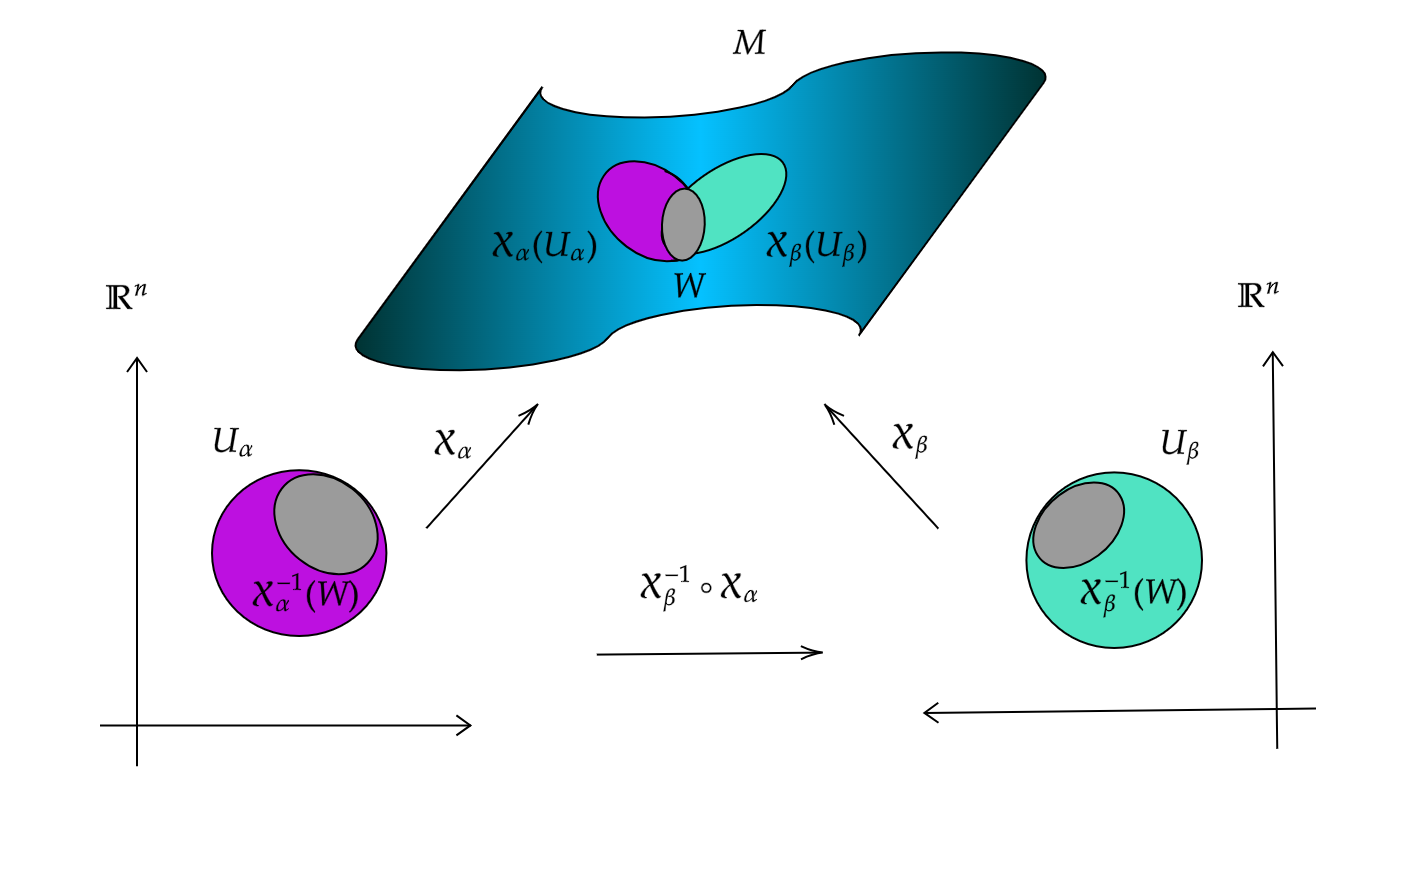
\includegraphics[width=\textwidth]{capitulos/variedaddif.png}
\end{figure}
\section{Funciones Diferenciables}

\begin{definition}
Dada $\varphi\colon M_1^n\to M_2^m$ se dice \textit{\textbf{diferenciable}} en $p\in M_1^n$ si, dada una parametrizaci\'on $\mathbf{y}$ de mi entorno de $\varphi(p)$, existe una parametrizaci\'on $\mathbf{x}$ de un entorno $U$ de $p$ tal que
\begin{equation*}
    \hat{\varphi}_{\mathbf{xy}}:=\mathbf{y}^{-1}\circ\varphi\circ\mathbf{x}\colon U\subseteq\mathbb{R}^n\to\mathbb{R}^m
\end{equation*}
sea diferenciable.
\end{definition}

\begin{theorem}
La definici\'on de diferenciabilidad est\'a bien dada (no depende de la elecci\'on de $\mathbf{x}$,$\mathbf{y}$).
\end{theorem}
\begin{proof}[\textbf{Demostraci\'on}]
Necesitamos demostrar que $\hat{\varphi}_{\mathbf{xy}}\in C^{\infty}$ si y solo si $\hat{\varphi}_{\tilde{\mathbf{x}}\tilde{\mathbf{y}}}$.
Para ello, notemos que 
\begin{align*}
    \hat{\varphi}_{\mathbf{xy}}&=\mathbf{y}^{-1}\circ\varphi\circ\mathbf{x}\\
    &=\underbrace{\mathbf{y}^{-1}\circ\tilde{\mathbf{y}}}_{C^\infty}\circ\underbrace{\tilde{\mathbf{y}}^{-1}\circ\varphi\circ\tilde{\mathbf{x}}}_{\hat{\varphi}_{\tilde{\mathbf{x}}\tilde{\mathbf{y}}}}\circ\underbrace{\tilde{\mathbf{x}}^{-1}\circ\mathbf{x}}_{C^\infty}.
\end{align*}
Notemos que, la igualdad anterior demuestra que $\hat{\varphi}_{\mathbf{xy}}\in C^{\infty}$ si y solo si $\hat{\varphi}_{\tilde{\mathbf{x}}\tilde{\mathbf{y}}}\in C^{\infty}$.
\end{proof}

\begin{definition}
$\hat{\varphi}_{\mathbf{xy}}$ se llama \textit{\textbf{representaci\'on en coordenadas}} de $\varphi$.    
\end{definition}

\begin{notation}
Cuando se escriba
\begin{equation*}
    \varphi(x^1,\dots,x^n)=\Bigl(\varphi^1(x^1,\dots,x^n),\dots,\varphi^m(x^1,\dots,x^n)\Bigl),
\end{equation*}
se entender\'a entonces que
\begin{equation*}
    \hat{\varphi}_{\mathbf{xy}}(x^1,\dots,x^n)=\Bigl(\hat{\varphi}_{\mathbf{xy}}^1(x^1,\dots,x^n),\dots,\hat{\varphi}_{\mathbf{xy}}^m(x^1,\dots,x^n)\Bigl).
\end{equation*}
\end{notation}

\begin{definition}
Decimos que $f\colon M_1\to M_2$ es un \textit{\textbf{difeomorfismo}} si $f\in C^\infty$ y si existe $f^{-1}$ tal que $f^{-1}\in C^\infty$   
\end{definition}

\begin{observation}
Regresando a las preguntas de la secci\'on 6.3, dados los modelos:
    \begin{enumerate}[label=(\alph*)]
        \item $p_1(x;\theta)=p(x;\mu,\sigma)=\frac{1}{\sqrt{2\pi}\sigma}e^{-\frac{1}{2}\frac{(x-\mu)^2}{\sigma^2}},\quad x\in\mathbb{R}\text{ y }(\mu,\sigma)\in\mathbb{R}\times\mathbb{R}_+$
        \item $p_2(x;\eta)=p(x;\rho,\tau)=\frac{\tau}{\sqrt{2\pi}}e^{-\frac{1}{2}(x\tau-\rho\tau+1)^2},\quad x\in\mathbb{R}\text{ y }(\rho,\tau)\in\mathbb{R}\times\mathbb{R}_+$\\
        y con $\rho=\mu+\sigma$, $\tau=\frac{1}{\sigma}$.
    \end{enumerate}
¿Podemos afirmar que $p_1(x;\theta)=p_2(x;\eta)$?\\

\noindent\textbf{S\'I:} Utilizando la definici\'on de difeomorfismo, podemos decir que $p_1(x;\theta)=p_2(x;\eta)$ pues definen la misma variedad, 
siendo $\eta_1=\theta_1+\theta_2=\mu+\sigma$ y $\eta_2=1/\theta_2=1/\sigma$ es cambio de coordenadas correspondiente.
%pero una funci\'on es el cambio de coordenadas para la otra. 
\end{observation}

\section{El Espacio Tangente}
\begin{definition}[\textbf{Tentativa}]
Decimos que $w\in T_pM$ si existe $\gamma\colon(-\varepsilon,\varepsilon)\to M$ tal que $\gamma(0)=p$ y  $\gamma'(0)=w$, donde $T_pM$ representa el espacio tangente a $M$ en $p\in M$.   
\end{definition}

\begin{observation}
La definici\'on anterior no nos funciona por el momento, pues con la informaci\'on que tenemos, no podemos calcular $\gamma'(0)$.    
\end{observation}

\subsection*{Motivaci\'on para una Definici\'on Formal:}

\noindent En $\mathbb{R}^n$, tomemos la curva 
\begin{equation*}
    \gamma\colon(-\varepsilon,\varepsilon)\to\mathbb{R}^n
\end{equation*}
la cual, cumple que
\begin{align*}
    \gamma(0)&=(x^1(0),\dots,x^n(0))=p\\
    \gamma'(0)&=\Bigl((x^1)'(0),\dots,(x^n)'(0)\Bigl)=w.
\end{align*}
Ahora, si tomamos $f\colon U_p\subseteq\mathbb{R}^n\to\mathbb{R}$, podemos definir la \textit{\textbf{derivada direccional}} de la siguiente manera:
\begin{align*}
    w_p(f)=df_p(w)&=\frac{d}{dt}f\circ\gamma\Big|_{t=0}\\
    &=\frac{\partial f}{\partial x^i}\Big|_p(x^i)'(0)\\
    &=\underbrace{(x^i)'(0)\frac{\partial}{\partial x^i}}_{w_p}f\Big|_p.
\end{align*}
Notemos que esta propiedad es intr\'inseca, pues solo necesito definir coordenadas a partir de la variedad diferencial en la que estamos. Esta idea motiva a definir lo siguiente:

\begin{definition}
Sea $M$ una variedad diferenciable y $\gamma\colon(-\varepsilon,\varepsilon)\to M$ tal que $\gamma(0)=p$. Sea 
\begin{equation*}
    D_p=\{f\colon M\to\mathbb{R}\colon\text{$f$ es difernciable en $p$}\}.
\end{equation*}
Definimos el \textit{\textbf{vector tangente}} a $\gamma$ en $p$ (con $t=0$), como la funci\'on
\begin{equation*}
    \gamma'(0)\colon D_p\to\mathbb{R}
\end{equation*}
dada por 
\begin{equation*}
    \gamma'(0)(f)=\frac{d}{dt}f\circ\gamma\Big|_{t=0}.
\end{equation*}
Por lo tanto, $w$ un \textit{\textbf{vector tangente}} a $M$ en $p$, es un vector tangente a $\gamma$ en $t=0$ por alguna $\gamma\colon(-\varepsilon,\varepsilon)\to M$ tal que $\gamma(0)=p$.
\end{definition}

\begin{notation}
En coordenadas, expresaremos 
\begin{equation}
    w(f)=\underbrace{(x^i)'(0)}_{\gamma'(0)}\frac{\partial}{\partial x^i}f\Big|_{p=\gamma(0)}
\end{equation}
donde $\mathbf{x}\colon U\subseteq\mathbb{R}^n\to U_p\subseteq M$ es la parametrizaci\'on.
\end{notation}

\begin{observation}
Dada la notaci\'on anterior, tenemos las siguientes observaciones:
\begin{enumerate}[label=(\alph*)]
    \item Para la ecuaci\'on (7.1), si $w=\frac{\partial}{\partial x^i}$, entonces $w$ es tangente a la \textit{\textbf{curva coordenada}} $x^i$.
    \item Por la ecuaci\'on (7.1), vemos que la definici\'on de $w$ s\'olo depende de $\gamma(0)$ y $\gamma'(0)$.
    \item El espacio de todos los vectores tangentes a $M$ en $p$ llamado \textit{\textbf{espacio tangente}} a $M$ en $p$, indicado con $T_pM$, es un espacio vectorial de dimensi\'on $n$ y adem\'as ya conocemos la base coordenada $\{\frac{\partial}{\partial x^i}|_p\}$ conocida como la base asociada a la parametrizaci\'on $\mathbf{x}$.
\end{enumerate}    
\end{observation}

\section{Diferencial y Campos Vectoriales}

\begin{definition}
Sea $\varphi\colon M_1\to M_2$ y sean $p\in M_1$ y $v\in T_pM$. Definimos el \textit{\textbf{diferencial}} de $\varphi$ en $p$ como la funci\'on 
\begin{equation*}
    d\varphi_p\colon T_pM_1\to T_{\varphi(p)}M_2
\end{equation*}
dada por
\begin{equation*}
    d\varphi_p(v)=\frac{d}{dt}\varphi\circ\gamma\Big|_{t=0}
\end{equation*}
donde $\gamma$ es una curva tal que $\gamma(0)=p$ y $\gamma'(0)=v$.
\end{definition}

\begin{theorem}
El diferencial $d\varphi_p$ cumple las siguientes propiedades:
\begin{enumerate}
    \item[(i)] Es lineal,
    \item[(ii)] No depende de la elecci\'on de $\gamma$ en la clase $[\gamma]=v$. 
\end{enumerate}
\end{theorem}
\begin{proof}[\textbf{Idea para la Demostraci\'on}]
Tomemos la ecuaci\'on 
\begin{equation}
    d\varphi_p(v)=\frac{\partial\varphi^i}{\partial x^j}\Big|_p(x^j)'(0)=\mathbf{J}\varphi_p\cdot[v]
\end{equation}
donde 
\begin{equation*}
    [v]=\Bigl((x^1)'(0)\dots,(x^n)'(0)\Bigl).
\end{equation*}
\end{proof}

\begin{definition}
Un \textit{\textbf{campo vectorial}} $\mathbf{X}$ sobre $M$ es una funci\'on que asocia a todo punto $p\in M$ un vector tangente $\mathbf{X}(p)$ a $M$ en $p$.    
\end{definition}

\begin{definition}
Se llama \textit{\textbf{haz tangente}} de $M$ la variedad diferenciable de dimensi\'on $2n$ dada por 
\begin{equation*}
    TM=\bigcup_{p\in M}T_pM.
\end{equation*}
\end{definition}

\begin{observation}
En coordenadas, se tiene que $\mathbf{X}(p)=\mathbf{X}^i(p)\frac{\partial}{\partial x^i}$. Entonces,
\begin{equation}
    \mathbf{X}(p)(f)=\mathbf{X}^i(p)\frac{\partial}{\partial x^i}f=df_p(\mathbf{X}).
\end{equation}
\end{observation}

\begin{definition}
Dado $\mathbf{X}\in\mathfrak{X}(M)$, $\gamma$ se llama \textit{\textbf{curva integral}} (\textit{\textbf{trayectoria}}) de $\mathbf{X}$ si 
\begin{equation}
    \gamma'(t)=\mathbf{X}(\gamma(t)),\quad\forall t\in(-\varepsilon,\varepsilon)
\end{equation}
En coordenadas, se representa como:
\begin{align*}
    &\gamma(t)=\Bigl(x^1(t),\dots,x^n(t)\Bigl)\\
    \text{Sistema de E.D.O's}
    &\begin{cases}
    (x^1)'(t)=\mathbf{X}^1\Bigl(x^1(t),\dots,x^n(t)\Bigl)\\
    \vdots\\
    (x^n)'(t)=\mathbf{X}^n\Bigl(x^1(t),\dots,x^n(t)\Bigl)
    \end{cases}\\
    \text{Condici\'on Inicial: }
    &\gamma(0)=q\overset{\text{En coord.}}{\iff}x^i(0)=x_0^i
\end{align*}
\end{definition}

\begin{theorem}[\textbf{Existencia y Unicidad de Curvas Integrales}]
Dada $\mathbf{X}\in\mathfrak{X}(M)$ y dada $q\in M$ existe una \'unica curva $\gamma\colon(-\varepsilon,\varepsilon)\to M$ tal que $\gamma$ es la curva integral de $\mathbf{X}$ que pasa por $p$.    
\end{theorem}

%\begin{observation}[\textbf{Convenci\'on de Einstein}]
%Recordemos que seg\'un la Ecuaci\'on (7.3), dado $\mathbf{X}\in\mathfrak{X}(M)$, la convenci\'on de Einstein estar\'a expresada por
%\begin{align*}
%    \mathbf{X}_p(f)=\mathbf{X}^i(x)\frac{\partial}{\partial x^i}f\Big|_p=df_p(\mathbf{X}),\quad i\in\{1,2,\dots,n\}.
%\end{align*}
%En la siguiente secci\'on, daremos una generalizaci\'on de esta idea.
%\end{observation}

\section{Tensores}

\begin{observation}
En la secci\'on anterior, vimos que dada una variedad diferenciable $M$ y dado $p\in M$, 
$T_pM$ es un espacio vectorial de dimensi\'on $n$. Seguiremos esta misma idea para escribir la siguente definici\'on.   
\end{observation}

\begin{definition}
Llamamos \textit{\textbf{espacio cotangente}} de $M$ en $p$ al conjunto dado por 
\begin{align*}
    T_p^{*}M=(T_pM)^{*}=\{f\colon T_pM\to\mathbb{R}|\text{$f$ es lineal}\}
\end{align*}
Sus elementos se llaman \textit{\textbf{covectores}} o \textit{\textbf{1-formas}}.
\end{definition}

\begin{example}
Sea $f\colon M\to\mathbb{R}$ tal que $f\in C^\infty$. Entonces $df_p\colon T_pM\to\mathbb{R}$ es lineal. De esta manera, $df_p\in T_p^{*}M$. En particular, si $\mathbf{x}\colon U\subseteq\mathbb{R}^n\to M$ es una parametrizaci\'on, se tendr\'a que $dx^i\in T_p^{*}M$.   

Resulta que $\{dx_p^i\}_{i=1}^{n}$ es una \textit{\textbf{base coordenada}} de $T_p^{*}M$ y adem\'as es la base dual de $\{\frac{\partial}{\partial x^j}|_p\}$ en el sentido de que, por la Ecuaci\'on (7.3), se tiene que 
\begin{equation*}
    dx^i\left(\frac{\partial}{\partial x^j}\right)=\frac{\partial}{\partial x^j}(x^i)=\delta_j^i.
\end{equation*}
\end{example}

\begin{definition}
Decimos que 
\begin{equation*}
    T^*M:=\bigcup_{p\in M}T_p^{*}M 
\end{equation*}
se llama el \textit{\textbf{haz cotangente}} de $M$ y es una variedad diferenciable de dimensi\'on $2n$ 
(con coordenadas locales $(x^i,\alpha_i)$).
\end{definition}

\begin{observation}
En general, una 1-forma $\alpha$ la puedo escribir en coordenadas como:
\begin{equation*}
    \alpha=\alpha_idx^i
\end{equation*}
\end{observation}

\begin{observation}
Dado un espacio vectorial $V$ finito-dimensional, sabemos que $(V^*)^*=V$. Esto nos dice que 
\begin{equation*}
    T_pM=\{f\colon T_p^{*}M\to\mathbb{R}\text{ lineales }\}.
\end{equation*}
\end{observation}

\begin{definition}
Decimos que 
\begin{equation*}
    \mathcal{T}_p^{(r,s)}M:=\Biggl\{f\colon\underbrace{T_p^{*}M\times\cdots\times T_p^{*}M}_{\text{$r$-veces}}\times\underbrace{T_pM\times\cdots\times T_pM}_{\text{$s$-veces}}\to\mathbb{R}\Bigg|\text{$f$ es lineal}\Biggl\}
\end{equation*}
se llama \textit{\textbf{espacio de los tensores}} de tipo $(r,s)$ de $M$ en $p$. Sus elementos se llaman \textit{\textbf{tensores}} de tipo $(r,s)$ en $p$.
\end{definition}

\begin{example}
Dada la definici\'on anterior, obtenemos las siguientes observaciones:
\begin{enumerate}
    \item[(i)] Los vectores de $T_pM$ son tensores de tipo $(1,0)$.
    \item[(ii)] Los covectores son tensores de tipo $(0,1)$ (1-formas).
\end{enumerate}
\end{example}

\begin{definition}
La variedad diferenciable 
\begin{equation*}
    \mathcal{T}^{(r,s)}:=\bigcup_{p\in M}\mathcal{T}_p^{(r,s)}M
\end{equation*}
se llama \textit{\textbf{haz de los tensores}} de tipo $(r,s)$.
\end{definition}

\begin{definition}
Dado $A\in\mathcal{T}^{(n,m)}M$ y $B\in\mathcal{T}^{(r,s)}M$, se define el \textit{\textbf{producto tensorial}} de $A$ y $B$ como el tensor 
\begin{equation*}
    A\otimes B\in\mathcal{T}^{(n+r,m+s)}M
\end{equation*}
dado por 
\begin{align*}
    &A\otimes B(\alpha_1,\dots,\alpha_{n+r},v_1,\dots,v_{m+s})\\
    &:=A(\alpha_1,\dots,\alpha_n,v_1,\dots,v_m)B(\alpha_{n+1},\dots,\alpha_{n+r},v_{m+1},\dots,v_{m+s}).
\end{align*}
\end{definition}

\begin{observation}
Dada $\mathbf{x}\colon U\subseteq\mathbb{R}^n\to M$ parametrizaci\'on, tenemos la \textit{\textbf{base coordenada}} (\textit{\textbf{base asociada}}) de $\mathcal{T}_p^{(r,s)}M$ dada por
\begin{equation*}
    \frac{\partial}{\partial x^{i_1}}\otimes\cdots\otimes\frac{\partial}{\partial x^{i_n}}\otimes dx^{j_1}\otimes\cdots\otimes dx^{j_s}
\end{equation*}
para 
\begin{align*}
    i_1&=1,\dots,n\\
    &\vdots\\
    i_r&=1,\dots,n\\
    j_1&=1,\dots,n\\
    &\vdots\\
    j_s&=1,\dots,n.
\end{align*}
En general, un tensor $\tau\in\mathcal{T}_p^{(r,s)}M$ se va a ver como 
\begin{align*}
    \tau=\tau^{i_1\dots i_n}_{j_1\dots j_s}    \frac{\partial}{\partial x^{i_1}}\otimes\cdots\otimes\frac{\partial}{\partial x^{i_n}}\otimes dx^{j_1}\otimes\cdots\otimes dx^{j_s}
\end{align*}
donde $\tau^{i_1\dots i_n}_{j_1\dots j_s}$ es la componente de $\tau$ en la base coordenada de $\mathcal{T}_p^{(r,s)}M$.
\end{observation}

\begin{example}
De los conceptos anteriores, podemos obtener los siguientes ejemplos:
\begin{enumerate}
    \item[(i)] Si $v$ es un tensor de tipo $(1,0)$, entonces
    \begin{equation*}
        v=v^i\frac{\partial}{\partial x^i},\quad([v]^i=v^i).
    \end{equation*}
    \item[(ii)] Si $\alpha$ es una tensor de tipo $(0,1)$, entonces
    \begin{equation*}
        \alpha=\alpha_idx^i,\quad([\alpha]_i=\alpha_i).
    \end{equation*}
    \item[(iii)] Si $g$ es un tensor de tipo (0,2), entonces
    \begin{equation*}
        g=g_{ij}dx^i\otimes dx^j,\quad([g]_{ij}=g_{ij}).
    \end{equation*}
\end{enumerate}
\end{example}

\begin{observation}[\textbf{Importante}]
Con la informaci\'on anterior, podemos hacer las siguientes preguntas:
\begin{enumerate}
    \item[(i)] ¿C\'omo calcular las componentes de un tensor en una base?
    \item[(ii)] ¿C\'omo cambian las componentes al cambiar de base?
\end{enumerate}
\end{observation}

\noindent\textbf{Respuestas:}
\begin{itemize}
    \item Para $v$ de tipo $(1,0)$, se tiene en coordenadas que
    \begin{equation*}
        v=v^i\frac{\partial}{\partial x^i}.
    \end{equation*}
    \begin{enumerate}
        \item[(i)] $v^i=v(x^i)\quad\|\quad\tilde{v}^j=v(\tilde{x}^j)$.
        \item[(ii)] Se tiene la siguiente ecuaci\'on:
        \begin{equation}
            \tilde{v}^j=v^i\frac{\partial}{\partial x^i}(\tilde{x}^j)=\frac{\partial\tilde{x}^j}{\partial x^i}v^i.
        \end{equation}
    \end{enumerate}
    Se dice que un tensor de tipo $(1,0)$ tiene 1 \textit{\textbf{\'indice contravariante}}.
    \item Para $\alpha$ de tipo $(0,1)$, se tiene en coordenadas que 
    \begin{equation*}
        \alpha=\alpha_idx^i.
    \end{equation*}
    \begin{enumerate}
        \item[(i)] $\alpha_i=\alpha\left(\frac{\partial}{\partial x^i}\right)\quad\|\quad\tilde{\alpha}_j=\alpha\left(\frac{\partial}{\partial\tilde{x}^j}\right)$.
        \item[(ii)] Se tiene la siguiente ecuaci\'on:
        \begin{equation}
            \tilde{\alpha}_j=\alpha_idx^i\left(\frac{\partial}{\partial\tilde{x}^j}\right)=\frac{\partial x^i}{\partial\tilde{x}^j}\alpha_i.
        \end{equation}
    \end{enumerate}
     Se dice que un tensor de tipo $(0,1)$ tiene 1 \textit{\textbf{\'indice covariante}}.
     \item Para $g$ de tipo $(0,2)$ se tiene en coordenadas que 
     \begin{equation*}
         g=g_{ij}dx^i\otimes dx^j.
     \end{equation*}
     \begin{enumerate}
         \item[(i)] $g_{ij}=g\left(\frac{\partial}{\partial x^i},\frac{\partial}{\partial x^j}\right)\quad\|\quad\tilde{g}_{rs}=g\left(\frac{\partial}{\partial\tilde{x}^r},\frac{\partial}{\partial\tilde{x}^s}\right)$.
         \item[(ii)] Se tiene la siguiente ecuaci\'on:
         \begin{equation}
             \tilde{g}_{rs}=g\left(\frac{\partial}{\partial\tilde{x}^r},\frac{\partial}{\partial\tilde{x}^s}\right)=g_{ij}dx^i\otimes dx^j\left(\frac{\partial}{\partial\tilde{x}^r},\frac{\partial}{\partial\tilde{x}^s}\right)=g_{ij}\frac{\partial x^i}{\partial\tilde{x}^r}\frac{\partial x^j}{\partial\tilde{x}^s}.
         \end{equation}
     \end{enumerate}
          Se dice que un tensor de tipo $(0,2)$ tiene 2 \textit{\textbf{\'indices covariantes}}.
\end{itemize}

\begin{observation}
A las ecuaciones (7.5), (7.6) y (7.7) las podemos ver como definiciones de tensor.   
\end{observation}

\begin{example}
Dada $f\colon M\to\mathbb{R}$ y dada $\mathbf{x}\colon U\subseteq\mathbb{R}^n\to M$ parametrizaci\'on, podemos definir $\partial f$ cuyas componentes en la base coordenada son
\begin{equation*}
    [\partial f]=\left(\frac{\partial f}{\partial x^1},\dots,\frac{\partial f}{\partial x^n}\right)
\end{equation*}
 y me pregunto si son las componentes de alg\'un tensor, por ejemplo, si son las componentes de un campo vectorial (el gradiente de $f$).
\end{example}

\begin{theorem}
La definici\'on de $\partial f$, cumple los siguientes incisos:
\begin{enumerate}[label=(\alph*)]
    \item No es un campo vectorial.
    \item Es una 1-forma.
    \item $\partial f=df$
\end{enumerate}
\end{theorem}
\begin{proof}[\textbf{Demostraci\'on}]
\begin{enumerate}[label=(\alph*)]
    \item Por definici\'on, se tiene que 
    \begin{equation*}
        v^i=\frac{\partial f}{\partial x^i}\quad\|\quad\tilde{v}^j=\frac{\partial f}{\partial\tilde{x}^j}
    \end{equation*}
    pero 
    \begin{equation*}
        \tilde{v}^i=\frac{\partial f}{\partial\tilde{x}^i}=\frac{\partial x^j}{\partial\tilde{x}^i}\frac{\partial f}{\partial x^j}=\frac{\partial x^j}{\partial\tilde{x}^i}v^j
    \end{equation*}
    \item Notemos que
    \begin{equation*}
        \alpha_i=\frac{\partial f}{\partial x^i}\quad\text{y}\quad\tilde{\alpha}_i=\frac{\partial x^j}{\partial\tilde{x}^i}\alpha_j
    \end{equation*}
    \item Por \'ultimo, observemos que 
    \begin{equation*}
        (\partial f)_i=\frac{\partial f}{\partial x^i}=\alpha_i
    \end{equation*}
    lo cual, implica que
    \begin{equation*}
        \alpha=\partial f=\frac{\partial f}{\partial x^i}dx^i=df.
    \end{equation*}
\end{enumerate}    
\end{proof}

\section{M\'etricas Riemannianas}

\begin{definition}
Una \textit{\textbf{m\'etrica riemanniana}} en $M$ es un campo tensorial $g$ de tipo $(0,2)$ tal que $\forall p\in M$, $g_p$ 
es un producto escalar euclideano en $T_pM$ (bilineal, sim\'etrico y definido positivo).
\end{definition}

\begin{notation}
La definici\'on anterior justifica la siguiente notaci\'on:
\begin{align*}
    g_p(v_1,v_2)&=\langle v_1,v_2\rangle\\
    g(\mathbf{X},\mathbf{Y})&=\langle \mathbf{X},\mathbf{Y}\rangle.
\end{align*}
\end{notation}

\noindent\textbf{En Coordenadas:} Sean 
\begin{equation*}
    g_{ij}(x)=g\left(\frac{\partial}{\partial x^i},\frac{\partial}{\partial x^j}\right)
\end{equation*}
y sean
\begin{equation*}
    \mathbf{X}=\mathbf{X}^i(x)\frac{\partial}{\partial x^i}\quad\text{y}\quad\mathbf{Y}=\mathbf{Y}^j(x)\frac{\partial}{\partial x^j}.
\end{equation*}
Esto implica que 
\begin{equation*}
    g(\mathbf{X},\mathbf{Y})=\mathbf{X}^i(x)\mathbf{Y}^j(x)g_{ij}(x)=\mathbf{X}^i\mathbf{Y}^jg_{ij}
\end{equation*}

\begin{definition}
Sea $f\colon M_1\to(M_2,g_2)$ diferenciable. Se le llama \textit{\textbf{pullback}} de $g_2$ con $f$ la m\'etrica en $M_1$ dada por
\begin{equation*}
    (f^*g_2)_p(v_1,v_2):=g_{2{f(p)}}(df_p(v_1),df_p(v_2)).
\end{equation*}
En coordenadas, se puede ver que:
\begin{equation*}
    (f^*g_2)_{ij}=\frac{\partial f^r}{\partial x^i}\frac{\partial f^s}{\partial x^j}(g_2)_{rs}.
\end{equation*}
\end{definition}

\begin{definition}
Sea $f\colon M_1\to(M_2,g_2)$ una inmersi\'on ($df_p$ es inyectiva), entonces a $f^*g_2$ le llamamos la \textit{\textbf{m\'etrica inducida}} por $f$ en $M_1$.   
\end{definition}


\begin{definition}
Se dice que $f\colon (M_1,g_1)\to(M_2,g_2)$ es \textit{\textbf{isometr\'ia}} si $f$ es un difeomorfismo y $f^*g_2=g_1$.    
\end{definition}


\begin{example}
Siguiendo las definiciones de esta secci\'on, tenemos los siguientes resultados:
\begin{enumerate}
    \item[(1)] \textbf{Geomet\'ia Euclideana ($R=0$):} $(\mathbb{R}^n,g^{std})$
    \begin{equation*}
        g^{std}=dx^1\otimes dx^1+\cdots+dx^n\otimes dx^n=\delta_{ij}dx^i\otimes dx^j.
    \end{equation*}
    \item[(2)] \textbf{Geometr\'ia Esf\'erica ($R=1$):} $\bigl(\mathbb{S}^{n-1},f^*g^{std}=g_{\mathbb{S}^{n-1}}^{std}\bigl)$ con $f\colon\mathbb{S}^{n-1}\to\mathbb{R}^n$ dada por
    \begin{align*}
        f^a&=x^a,\quad a=1,2,\dots,n-1\\
        f^n&=\sqrt{1-\sum_{i=1}^{n-1}(x^i)^2}
    \end{align*}
    \begin{equation*}
        g_{\mathbb{S}^{n-1}}^{std}=\left(\delta_{ab}+\frac{x^ax^b}{1-\sum_{i=1}^{n-1}(x^i)^2}\right)dx^a\otimes dx^b,\quad a,b=1,2,\dots,n-1. 
    \end{equation*}
    \item[(3)] \textbf{Geometr\'ia Hiperb\'olica ($R=-1$):} $(\mathbb{R}\times\mathbb{R}_+,g^p)$ donde $(x,y)\in\mathbb{R}\times\mathbb{R}_+$
    \begin{equation*}
        g^p:=\frac{1}{y^2}(dx\otimes dx+dy\otimes dy).
    \end{equation*}
\end{enumerate}    
\end{example}
    \chapter{Geometr\'ia de la \\
    Informaci\'on}
    En este cap\'itulo, daremos una breve introducci\'on a la Geometr\'ia de la Informaci\'on a partir de los puntos que se mencionaron en el cap\'itulo 6:

\begin{enumerate}[label=(\alph*)]
        \item Generalizaci\'on de la Geometr\'ia Riemanniana
        \item Aplicaciones:
        \begin{itemize}
            \item Divergencias en T.D.A.
            \item Principio de M\'axima Entrop\'ia en Termodin\'amica (Induce a la Geometr\'ia Dual)
            \item $f$-Divergencias + D.P.I. tienen como consecuencia el Teorema de Chentsov
        \end{itemize}
\end{enumerate}

\section{M\'etrica en la\\
Geometr\'ia de la Informaci\'on}
\begin{theorem}
Dado $p(x;\theta)$ modelo estad\'istico $x\in\mathcal{X}$ y $\theta\in\Theta$ tenemos que 
\begin{equation*}
    \mathcal{I}_{ij}(\theta)=\mathbb{E}_{p(x;\theta)}\left[\frac{\partial\ell}{\partial \theta^i}\cdot\frac{\partial\ell}{\partial\theta^j}\right],\quad\ell=\ln{p(x;\theta)}
\end{equation*}
define una m\'etrica riemanniana en $\Theta$ dada por
\begin{equation*}
    g^F(\theta):=\mathcal{I}_{ij}(\theta)d\theta^i\otimes d\theta^j
\end{equation*}
\end{theorem}

\begin{proof}[\textbf{Demostraci\'on}]
\begin{enumerate}
    \item[(i)] $\mathcal{I}_{ij}(\theta)$ son las componentes de un tensor de tipo (0,2) porque
    \begin{equation*}
        g^F(\theta)=\mathbb{E}_{p(x;\theta)}\left[d\ell\otimes d\ell\right].
    \end{equation*}
    \item[(ii)] $\mathcal{I}_{ij}(\theta)\succeq0$ pues sabemos, por definici\'on, que es una matriz de covarianza.
\end{enumerate}
\end{proof}

\begin{example}
Con el teorema anterior, se pueden comprobar los siguientes resultados:
\begin{enumerate}
    \item[(1)] \textbf{Geometr\'ia Hiperb\'olica:} Sea $p(x;\theta)=\frac{1}{\sqrt{2\pi}\sigma}e^{-\frac{(x-\mu)^2}{\sigma^2}}$ con $\Theta=\mathbb{R}\times\mathbb{R}_+$ y $(\mu,\sigma)\in\Theta$. Se puede probar que esto nos lleva a un modelo estad\'istico para la geometr\'ia hiperb\'olica, pues
    \begin{align*}
    g_{11}^F(\mu,\sigma)&=\frac{1}{\sigma^2}\\
    g_{12}^F(\mu,\sigma)&=0\\
    g_{22}^F(\mu,\sigma)&=\frac{2}{\sigma^2}
    \end{align*}
    \begin{equation*}
        \Longrightarrow g^F=\frac{1}{\sigma^2}(d\mu\otimes d\mu+2d\sigma\otimes d\sigma).
    \end{equation*}
    \item[(2)] \textbf{Geometr\'ia Esf\'erica:} En $\mathbb{S}_{n-1}$ tenemos $\mathcal{X}=\{1,\dots,n\}$ y $\mathbb{P}(X=i)=p_i>0$. 
    Entonces, parametricemos $\mathbb{S}_{n-1}$ por $\theta^i=\sqrt{p_i}$. Luego, se puede probar lo siguiente:
    \begin{enumerate}
        \item[(i)] $\theta^i>0$ con $\sum_{i=1}^{n}(\theta^i)^2=1$,  %\Longrightarrow \Theta=\frac{1}{4}\mathbb{S}^{n-1}$,
%        \begin{equation*}
%          
%        \end{equation*}
        es decir, $\mathbb{S}_{n-1}$ es el octante positivo de la esfera. 
        \item[(ii)] Se tiene que 
        \begin{align*}
            g_{ij}^F(\theta)&=\sum_{k=1}^{n}(\theta^k)^2\frac{\partial}{\partial\theta^i}\ln(\theta^k)^2\frac{\partial}{\partial\theta^j}\ln(\theta^k)^2\\
            &=4\delta_{ij}\big|_{\mathbb{S}^{n-1}}=4g_{\mathbb{S}^{n-1}}^{std}
        \end{align*}
    \end{enumerate}
    \item[(3)] \textbf{Geometr\'ia Euclideana:} Sea $p(x;\theta)=\exp(\theta^ih_i(x)-\psi(\theta))$ con
    \begin{equation*}
        \psi(\theta):=\ln\int_{\mathcal{X}}\exp(\theta^ih_i(x))dx.
    \end{equation*}
    \begin{equation*}
        (\text{Modelo Exponencial})
    \end{equation*}
    Se puede probar que 
    \begin{equation*}
        g^F(\theta)=\frac{\partial^2\psi}{\partial\theta^i\partial\theta^j}d\theta^i\otimes d\theta^j.
    \end{equation*}
    En el caso de que $\psi(\theta)=\sum_{i=1}^{n}f_i(\theta^i)$, entonces obtendremos un modelo estad\'istico para la Geometr\'ia Euclideana. 
\end{enumerate}

\end{example}

\begin{observation}
Podemos ver que, el conc\'epto de m\'etrica en la geometr\'ia de la informaci\'on, al igual que en geometr\'ia Riemanniana, 
nos permite definir los siguientes conceptos:
\begin{itemize}
    \item Longitudes
    \item \'Angulos
    \item Vol\'umenes
    \item Gradientes
\end{itemize}
Sin embargo, en la geometr\'ia de la informaci\'on, requerimos de m\'as herramientas adem\'as de $g$ para poder definir:
\begin{itemize}
    \item Curvatura
    \item Geod\'esicas
\end{itemize}
\end{observation}

\begin{definition}
Sea $\gamma\colon I=(a,b)\subset\mathbb{R}\to(M,g)$ una curva. 
Sea $\frac{d\gamma}{dt}$ su vector tangente. Definimos la \textit{\textbf{longitud}} de $\gamma$ como el n\'umero
\begin{align*}
    l(\gamma):=\int_a^b\sqrt{g\left(\frac{d\gamma}{dt},\frac{d\gamma}{dt}\right)}dt=\int_a^b\sqrt{g_{ij}(x)\dot{x}^i\dot{x}^j}dt.
\end{align*}
\end{definition}

\begin{definition}
Sea $R\subseteq(M,g)$ una regi\'on cuya cerradura es compacta y tal que $R\subseteq\mathbf{x}(U)$. Definimos el \textit{\textbf{vol\'umen}} de $R$ como 
\begin{equation*}
    \text{Vol}(R):=\int_{\mathbf{x}^{-1}(R)}\sqrt{\text{det}(g)}dx^1\cdots dx^n.
\end{equation*}
\end{definition}

\begin{observation}
Se puede ver que $l(\gamma)$ y $\text{Vol}(R)$ no dependen de las coordenadas, es decir, est\'an bien definidas.     
\end{observation}

\begin{example}
La \textit{\textbf{prior de Jeffrey}} en estad\'istica Bayesiana es la distribuci\'on
\begin{equation*}
    f(\theta)=\sqrt{\text{det}\mathcal{I}_{ij}(\theta)}=\sqrt{\text{det}g^F(\theta)}.
\end{equation*}
De las definiciones anteriores vemos que entonces la prior de Jeffrey corresponde al elemento de
volumen invariante en el espacio de par\'ametros de un modelo estad\'istico definido por la m\'etrica de Fisher.
\end{example}

\begin{example}
Se define la \textit{\textbf{energia de una curva}} como
\begin{equation*}
    E(\gamma)=\int_a^bg(\gamma,\gamma)dt.
\end{equation*}
Se puede probar que $E(\gamma)\geq \frac{1}{b-a}l(\gamma)^2$.
\end{example}

\section{Estad\'isticas Suficientes}

\begin{definition}
Sea $p(x;\theta)$ un modelo estad\'istico y sea $y=k(x)$ una funci\'on (que puede ser muchos a 1) y sea
\begin{equation*}
    K_p(y;\theta):=\sum_{x\colon k(x)=y}p(x;\theta).
\end{equation*}
Decimos que $k(x)$ es un \textit{\textbf{estad\'istico suficiente}} para $\theta$ si 
\begin{equation*}
    p(x;\theta)=K_p(y;\theta)h(x).
\end{equation*}
\end{definition}

\begin{theorem}[\textbf{Chentsov. 1974}~\cite{chentsov1982statiscal}]
En $\mathbb{S}_{n-1}$ se cumplen los siguientes enunciados:
\begin{enumerate}
    \item[(i)] $g^F(\theta)$ es invariante por estad\'isticos suficientes.
    \item[(ii)] Si $g(\theta)$ es una m\'etrica invariante por estad\'isticos suficientes
    \begin{equation*}
        \Longrightarrow g(\theta)=c\cdot g^F(\theta),
    \end{equation*}
    con $c\in\mathbb R$ una constante.
\end{enumerate}
\end{theorem}

\begin{observation}
Podemos notar lo siguiente:
\begin{enumerate}
    \item[(1)] El teorema anterior, junto con las definiciones previas, termina de contestar la pregunta 2 de la secci\'on 6.3 de estas notas (existencia 
    y unicidad del concepto de distancia en $p(x;\theta)$).
    \item[(2)] Hay pruebas de extensiones de este teorema para el modelo exponencial y modelos exponenciales curvos~\cite{campbell1986extended,dowty2018chentsov}. 
    \item[(3)] Dentro de esta teor\'ia, se puede incluso probar que todo modelo es exponencial~\cite{brody2007note} y 
    entonces los puntos anteriores motivan sugerir que la m\'etrica de Fisher es \'unica para cualquier modelo estad\'istico.
\end{enumerate}
\end{observation}

\section{Conexiones Afines y Geod\'esicas}

\begin{theorem}
Dada $(M,g)$, $g_p$ induce un isomorfismo entre $T_pM$ y $T_p^*M$.    
\end{theorem}

Como idea para la demostraci\'on, podemos ver que, dado $v\in T_pM$, $\alpha_v:=g_p(v,\cdot)$. 
Luego, dada $\alpha\in T_pM$, $v^\alpha$ es el vector tal que 
\begin{equation*}
    \alpha_p=g_p(v^\alpha,\cdot)
\end{equation*}
En coordenadas, tenemos que 
\begin{align*}
    \alpha_v&=g_{ij}dx^i\otimes dx^j\left(v^r\frac{\partial}{\partial x^r},\cdot\right)\\
    &=g_{ij}v^rdx^i\left(\frac{\partial}{\partial x^r}\right)dx^j\\
    &=g_{ij}v^r\delta_r^idx^j=g_{ij}v^idx^j
\end{align*}
Se puede ver que $v^\alpha=g^{ij}\alpha_j\frac{\partial}{\partial x^i}$

\begin{example}[\textbf{Muy Importante}]
Dada $(M,g)$ y $f\colon M\to\mathbb{R}$, se tiene que $df_p\in T_p^*M$. Adem\'as 
\begin{equation*}
    df=\frac{\partial f}{\partial x^i}dx^i.
\end{equation*}
Entonces, usando el isomorfismo de arriba, tenemos que el \textbf{gradiente} de $f$, $\text{grad}_pf$, es el vector dado por
\begin{equation*}
    df_p=g_p(\text{grad}_pf,\cdot)\,.
\end{equation*}
En coordenadas, se tiene que 
\begin{equation*}
    \text{grad}f=g^{ij}\frac{\partial f}{\partial x^i}\frac{\partial}{\partial x^j}.
\end{equation*}
Como caso particular, podemos dar el siguiente: en $\mathbb{R}^n$
\begin{equation*}
    g^{std}=dx^1\otimes dx^1+\cdots+dx^n\otimes dx^n
\end{equation*}
y en coordenadas cartesianas $g^{ij}=\delta^{ij}$
\begin{equation*}
    \Longrightarrow\text{grad}f=\delta^{ij}\frac{\partial f}{\partial x^i}\frac{\partial}{\partial x^j}
\end{equation*}
recuperando entonces la noci\'on de gradiente usual en $\mathbb R^n$.
\end{example}

\begin{theorem}
Se tiene que $v^*$ satisface
\begin{equation*}
    v^*=\underset{\|v\|_g=1}{\text{arg}\max}\,df_p(v)\iff v^*=\frac{\text{grad}_pf}{\|\text{grad}_pf\|_g}
\end{equation*}
\end{theorem}

\noindent\textbf{En Conclusi\'on:} En $(M,g)$, si queremos optimizar $f$, tenemos que usar el \textbf{\textit{flujo gradiente riemanniano (natural)}}
\begin{equation*}
    \dot{\gamma}(t)=-\text{grad}_{\gamma(t)}f(\gamma(t))
\end{equation*}
lo cual es una definici\'on intr\'inseca, pues no depende de las coordenadas. 

En coordenadas, escribimos
\begin{equation}
    \dot{x}^i(t)=-g^{ij}(x(t))\frac{\partial f}{\partial x^j}(x(t))
\end{equation}

\begin{definition}
Una \textbf{\textit{conexi\'on af\'in}} en $M$ es un mapa $\nabla\colon\mathfrak{X}(M)\times\mathfrak{X}(M)\to\mathfrak{X}(M)$ tal que, $\forall X,Y,Z\in\mathfrak{X}(M)$ y $f,g\in C^{\infty}(M)$
\begin{enumerate}
    \item[(i)]\textbf{Linealidad 1:} $\nabla_{fX+gY}Z=f\nabla_XZ+g\nabla_YZ$.
    \item[(ii)]\textbf{Linealidad 2:} $\nabla_X(Y+Z)=\nabla_XY+\nabla_XZ$.
    \item[(iii)]\textbf{Leibniz:} $\nabla_X(fY)=f\nabla_XY+X(f)Y$
\end{enumerate}
\end{definition}

\noindent\textbf{En Coordenadas:} $X=X^i\frac{\partial}{\partial x^i}$ y $Y=Y^j\frac{\partial}{\partial x^j}$.
\begin{align*}
    \Longrightarrow\nabla_XY&=\nabla_{X^i\frac{\partial}{\partial x^i}}\left(Y^j\frac{\partial}{\partial x^j}\right)\\
    &=X^i\nabla_{\frac{\partial}{\partial x^i}}\left(Y^j\frac{\partial}{\partial x^j}\right)\\
    &=X^iY^j\underbrace{\nabla_{\frac{\partial}{\partial x^i}}\frac{\partial}{\partial x^j}}_{\Gamma_{ij}^k\frac{\partial}{\partial x^k}}+X^i\frac{\partial Y^j}{\partial x^i}\frac{\partial}{\partial x^j}\\
    &=\left(X^iY^j\Gamma_{ij}^k+X^i\frac{\partial Y^k}{\partial x^i}\right)\frac{\partial}{\partial x^k}
\end{align*}
\begin{equation}
    \Longrightarrow\nabla_XY=\left(X^iY^j\Gamma_{ij}^k+X^i\frac{\partial Y^k}{\partial x^i}\right)\frac{\partial}{\partial x^k}.
\end{equation}

En la serie de igualdades anteriores, se tiene que $\Gamma_{ij}^k$ son llamados \textit{\textbf{s\'imbolos de Christoffel}}, donde $\Gamma_{ij}^k\leftrightarrow\nabla$.

\begin{example}
Sea $\gamma$ una curva y sean $X=\dot{\gamma}$ y $Y=\dot{\gamma}$. De esta manera, 
\begin{equation*}
    \dot{\gamma}=\dot{x}^i\frac{\partial}{\partial x^i}.
\end{equation*}
Tenemos entonces que la ecuaci\'on
\begin{equation*}
    \nabla_{\dot{\gamma}}\dot{\gamma}=\left(\dot{x}^i\dot{x}^j\Gamma_{ij}^k+\ddot{x}^k\right)\frac{\partial}{\partial x^k}
\end{equation*}
se le conoce como la \textbf{\textit{aceleraci\'on}} de $\gamma$.
\end{example}

\begin{definition}
Las curvas con aceleraci\'on igual a cero se llaman \textit{\textbf{geod\'esicas}}.   
\end{definition}

\begin{observation}
Las ecuaciones para obtener las geod\'esicas son:
\begin{equation*}
    \ddot{x}^k+\dot{x}^i\dot{x}^j\Gamma_{ij}^k=0.
\end{equation*}
\end{observation}

\begin{definition}
Sea $(M,g)$ y sea $\nabla$ una conexi\'on af\'in. Decimos que $\nabla$ es \textit{\textbf{compatible}} con $g$ si
\begin{equation*}
    Z(g(X,Y))=g(\nabla_ZX,Y)+g(X,\nabla_ZY).
\end{equation*}
Decimos que $\nabla$ ($\leftrightarrow\Gamma_{ij}^k$) es \textbf{\textit{sim\'etrica}} si 
\begin{equation*}
    \Gamma_{ij}^k=\Gamma_{ji}^k,\quad\forall i,j,k=1,\dots,n.
\end{equation*}
\end{definition}

\begin{theorem}[\textbf{Fundamental de la Geometr\'ia Riemanniana}]
Sea $(M,g)$ variedad riemanniana. Entonces, existe una \'unica conexi\'on $\nabla_{LC}$ tal que:
\begin{enumerate}
    \item[(i)] $\nabla_{LC}$ es compatible con $g$.
    \item[(ii)] $\nabla_{LC}$ es sim\'etrica.
\end{enumerate}
donde a $\nabla_{LC}$ se le conoce como la conexi\'on de Levi-Civita.
\end{theorem}

\noindent\textbf{En Coordenadas:} ($\nabla\leftrightarrow\Gamma_{ij}^k$)
\begin{equation*}
\Gamma_{ij}^k=\frac{1}{2}g^{km}(g_{im,j}+g_{jm,i}-g_{ij,m})
\end{equation*}
donde $g_{im,k}=\frac{\partial}{\partial x^k}g_{im}$.

\begin{example}
$\mathbb{R}^n$, $g^{std}=g_{ij}dx^i\otimes dx^j=\delta_{ij}dx^i\otimes dx^j$ 
\begin{equation*}
    \Gamma_{ij}^k=0.
\end{equation*}
Entonces, las geod\'esicas de $(\mathbb{R}^n,g^{std})$ est\'an dadas por
\begin{equation*}
    \ddot{x}^k =0\,. %+\Gamma_{ij}^k\dot{x}^i\dot{x}^j=0.
\end{equation*}
Por lo tanto, est\'an dadas por rectas:
\begin{equation*}
    x^k(s)=a^ks+b^k,\quad a^k,b^k\in\mathbb{R}.
\end{equation*}
\end{example}

\begin{definition}
Sea $\nabla$ una conexi\'on en $M$. Definimos la \textbf{\textit{curvatura}} de $\nabla$ como el tensor (1,3) dado por
\begin{equation*}
    R^{\nabla}(X,Y,Z):=\nabla_X\nabla_YZ-\nabla_Y\nabla_XZ-\nabla_{[X,Y]}Z
\end{equation*}
donde 
\begin{equation*}
    [X,Y]:=XY-YX
\end{equation*}
es conocido como el \textit{\textbf{corchete de Lie}}
\end{definition}

\begin{observation}
Se puede demostrar que $[X,Y]$ es un campo vectorial.     
\end{observation}

\begin{definition}
$(M,\nabla)$ se dice \textbf{\textit{plana}} si $R^\nabla=0$.    
\end{definition}

\section{Generalizaci\'on de la\\
Geometr\'ia Riemanniana}

\begin{definition}
Sea $(M,g)$ variedad riemanniana y sean $\nabla$ y $\nabla^*$ dos conexiones afines sim\'etricas en $M$. Decimos que $\nabla$ y $\nabla^*$ son \textit{\textbf{duales}} con respecto a $g$ si 
\begin{equation*}
    Z(g(X,Y))=g(\nabla_ZX,Y)+g(X,\nabla_Z^*Y).
\end{equation*}
\end{definition}

\begin{observation}
Si $\nabla=\nabla^*$ entonces $\nabla=\nabla_{LC}$.    
\end{observation}

\begin{definition}
A $(M,g,\nabla,\nabla^*)$ se le llama \textit{\textbf{variedad estad\'istica}}.    
\end{definition}

\begin{theorem}[\textbf{Fundamental de la Geometr\'ia de la Informaci\'on}]\cite{nielsen2020elementary}
Dada $(M,g,\nabla)$, se cumplen los siguientes enunciados:
\begin{enumerate}
    \item[(i)] Existe una \'unica conexi\'on $\nabla^*$ dual de $\nabla$ con respecto de $g$.
    \item[(ii)] $R^\nabla=0$ si y solo si $R^{\nabla^*}=0$ (en este caso se dice que la variedad estad\'istica es \textbf{dualmente plana}).
\end{enumerate}
\end{theorem}

\begin{theorem}
Sea $D\colon M\times M\to\mathbb{R}$ una divergencia sobre $M$. Entonces $D$ induce la variedad estad\'istica $(M,g^D,\nabla^D,\nabla^{*D})$ dada por
\begin{align*}
    (g^D)_{ij}&=\frac{\partial}{\partial\theta_1^i}\frac{\partial}{\partial\theta_1^j}D\bigl(\theta(P_1)\|\theta(P_2)\bigl)\Big|_{\theta(P_1)=\theta(P_2)}\\
    (\Gamma^D)_{ijk}&=-\frac{\partial}{\partial\theta_1^i}\frac{\partial}{\partial\theta_1^j}\frac{\partial}{\partial\theta_2^k}D\bigl(\theta(P_1)\|\theta(P_2)\bigl)\Big|_{\theta(P_1)=\theta(P_2)}\\
    (\Gamma^{*D})_{ijk}&=-\frac{\partial}{\partial\theta_2^i}\frac{\partial}{\partial\theta_2^j}\frac{\partial}{\partial\theta_1^k}D\bigl(\theta(P_1)\|\theta(P_2)\bigl)\Big|_{\theta(P_1)=\theta(P_2)}.
\end{align*}
\end{theorem}

\begin{observation}
Si $D=D_f$, entonces $g^D=g^F$. Adem\'as, si estamos en la familia exponencial
\begin{equation*}
    \exp(\theta^ah_a(x)-\psi(\theta)).
\end{equation*}
Entonces, tenemos que 
\begin{equation*}
    g^F(\theta)=\frac{\partial^2\psi}{\partial\theta^a\partial\theta^b}d\theta^a\otimes d\theta^b.
\end{equation*}
y la variedad es dualmente plana.
\end{observation}

%\section{Aplicaciones a la\\
%F\'isica Estad\'istica}

%\subsection*{Motivaci\'on}
%En esta secci\'on, daremos solo una breve introducci\'on a las posibles aplicaciones de la Geometr\'ia de la Informaci\'on, entre las cuales, est\'a la F\'isica Estad\'isitica. Los puntos principales que nos servir\'an como motivaci\'on, ser\'an:
%\begin{itemize}
%    \item \textbf{Efecto Mpemba:} Congelaci\'on de agua caliente ocurre a mayor velocidad que la congelaci\'on de agua fr\'ia
%    \item \textbf{Relajaci\'on Asim\'etrica (Proceso Ornstein–Uhlenbeck):} Proceso estoc\'astico que estudia la velocidad de una particula Browniana bajo fricci\'on. 
%\end{itemize}

%En este caso, estudiaremos un sistema termodin\'amico a partir de modelos estad\'isticos con espacio fase
%\begin{equation*}
%    \Gamma:=(T^*Q)^N,\quad N\approx10^{23}
%\end{equation*}
%y una funci\'on 
%\begin{equation*}
%    \rho\colon\Gamma\to[0,1]
%\end{equation*}
%Si $x\in\Gamma$ se puede ver que 
%\begin{equation*}
%    \rho(x;\theta)=\exp(\theta^ah_a(x)-\psi(\theta))
%\end{equation*}
%lo cual forma una variedad dualmente plana en nuestro objeto de estudio. Utilizando la Geometr\'ia de la Informaci\'on, se ha propuesto el siguiente teorema:

%\begin{theorem}[\textbf{Amari}]
%Las soluciones de la ecuaci\'on
%\begin{equation*}
%    \dot{\gamma}(t)=-k\text{grad}_{\gamma(t)}D(q\|\gamma(t))
%\end{equation*}
%son $\nabla^*$-geod\'esicas que convergen a un punto de equilibrio $q$.
%\end{theorem}

%\begin{observation}
%Pedimos a la curva que su aceleraci\'on sea en su direcci\'on, es decir, 
%\begin{equation*}
%    \nabla_{\dot{\gamma}}\dot{\gamma}=-k\dot{\gamma}.
%\end{equation*}
%\end{observation}

%A partir de este tipo de teor\'ia junto con el Proceso Ornstein–Uhlenbeck, buscamos comprobar el efecto Mpemba, es decir, comprobar que el sistema caliente llega m\'as r\'apido al equilibrio $q$ que el sistema fr\'io. 
\bibliography{bibliografia}
\end{document}